 \documentclass[a4paper,12pt]{article}

\usepackage[ngerman]{babel}
\usepackage{amsmath}
\usepackage{amssymb}
\usepackage{graphicx}
\usepackage[a4paper,margin=2cm]{geometry}
\usepackage{float}
\usepackage{enumitem}
\usepackage{multicol}
\title{Ladung und Potential}
\author{}
\date{}

\begin{document}
	
	\maketitle
	\tableofcontents
	\pagebreak
	
	\section{Spule}
	
	\subsection{Flussverkettung}
	$$\psi = L \cdot I$$
	
	\subsection{Spannung}
	$$u = L \cdot \frac{dI}{dt}$$
	
	\subsection{Induktivität}
	$$L = \frac{\psi}{I}$$
	
	Zylinderspule:
	$$L = \mu_0 \cdot \frac{N^2 \cdot A}{l}$$
	
	\subsection{Gespeicherte magnetische Energie}
	$$W = \frac{1}{2} L I_0^2$$
	
	\subsection{Parallelschaltung}
	Bei der Parallelschaltung von Spulen addieren sich die Kehrwerte (analog Parallelschaltung Widerstände):
	$$\frac{1}{L_p} = \sum \frac{1}{L_i}$$
	
	\subsection{Serienschaltung}
	Bei der Serienschaltung von Spulen addieren sich die Induktivitäten (analog Serienschaltung Widerstände):
	$$L_s = \sum L_i$$
	
	\subsection{Verhalten einer Spule beim Schließen des Kreises}
	
	Eine Spule verhindert jede sprunghafte Änderung des Stroms, da gilt:
	\[
	u_L(t) = L \cdot \frac{di}{dt}
	\]
	Ein instantaner Stromanstieg würde $\frac{di}{dt} \to \infty$ und damit eine 
	unendlich große Spannung erfordern, was physikalisch nicht möglich ist.\\
	
	\textbf{Kurz vor dem Schließen} ($t < 0$):
	\hspace{1em} $i_L = 0$, \hspace{0.5em} $u_L = 0$\\
	
	\textbf{Kurz nach dem Schließen} ($t = 0^+$):
	\hspace{1em} $i_L = 0$ (unverändert), \hspace{0.5em} $u_L = U_{\text{Quelle}}$\\
	\hspace*{1em}$\Rightarrow$ Die Spule verhält sich wie ein \textit{offener Schalter}.\\
	
	\textbf{Im eingeschwungenen Zustand} ($t \to \infty$):
	\hspace{1em} $u_L = 0$, \hspace{0.5em} $i_L = \dfrac{U}{R}$\\
	\hspace*{1em}$\Rightarrow$ Die Spule verhält sich wie ein \textit{Kurzschluss}.
	
	\subsection{Laden und Entladen}
	
	\begin{tabular}{p{0.45\textwidth} p{0.45\textwidth}}
		\vspace{0pt}
		\textbf{Laden}
		$$u_C(t) = U_0 \left(1 - e^{-\frac{t}{\tau}}\right)$$
		$$i(t) = \frac{U_0}{R}\, e^{-\frac{t}{\tau}}$$
		&
		\vspace{0pt}
		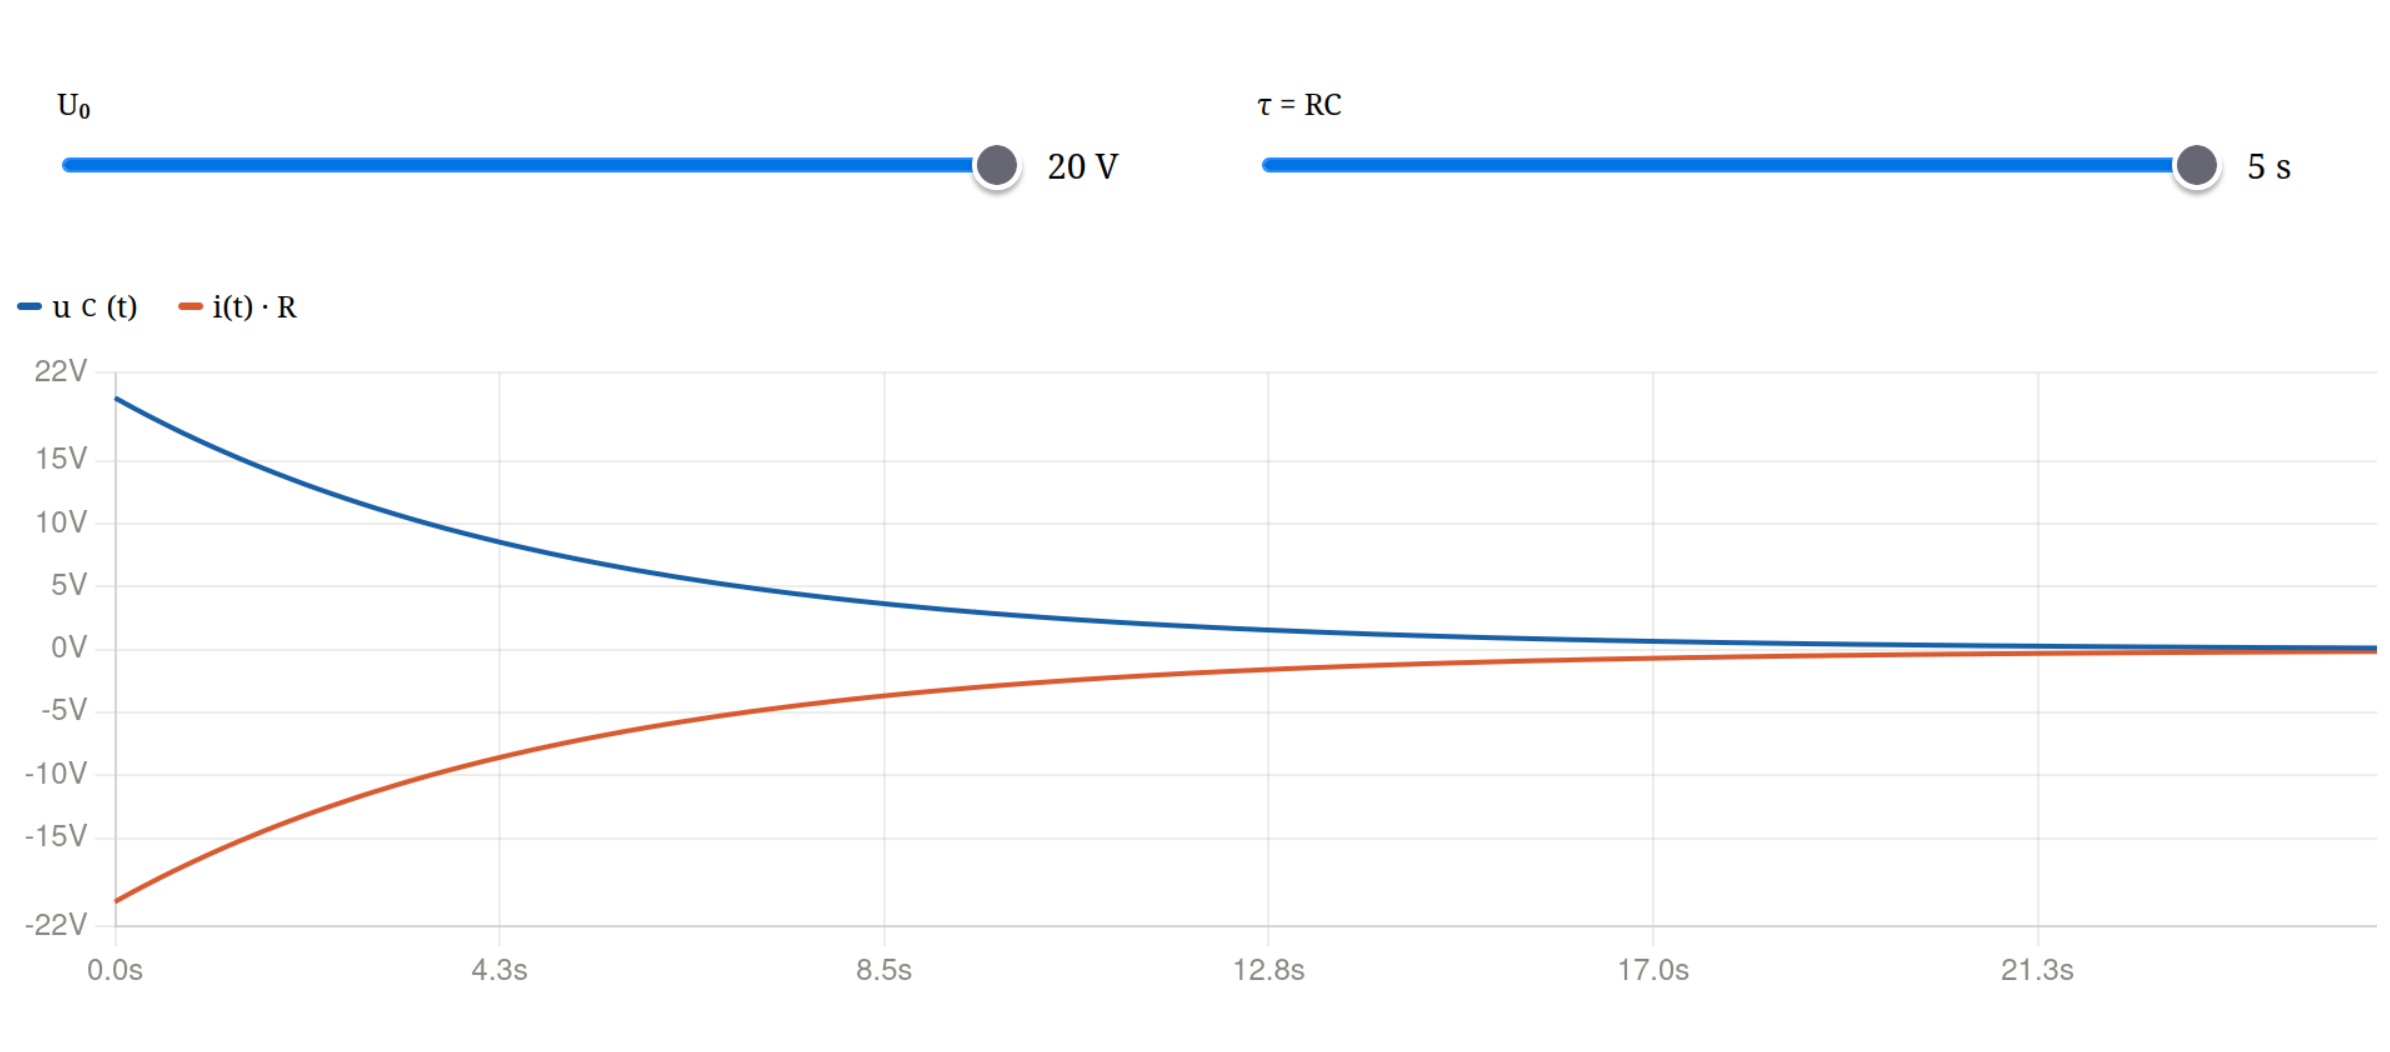
\includegraphics[width=0.5\textwidth]{img/spule_laden} \\
		
		\vspace{0pt}
		\textbf{Entladen}
		$$u_C(t) = U_0 \cdot e^{-\frac{t}{\tau}}$$
		$$i(t) = -\frac{U_0}{R}\, e^{-\frac{t}{\tau}}$$
		&
		\vspace{0pt}
		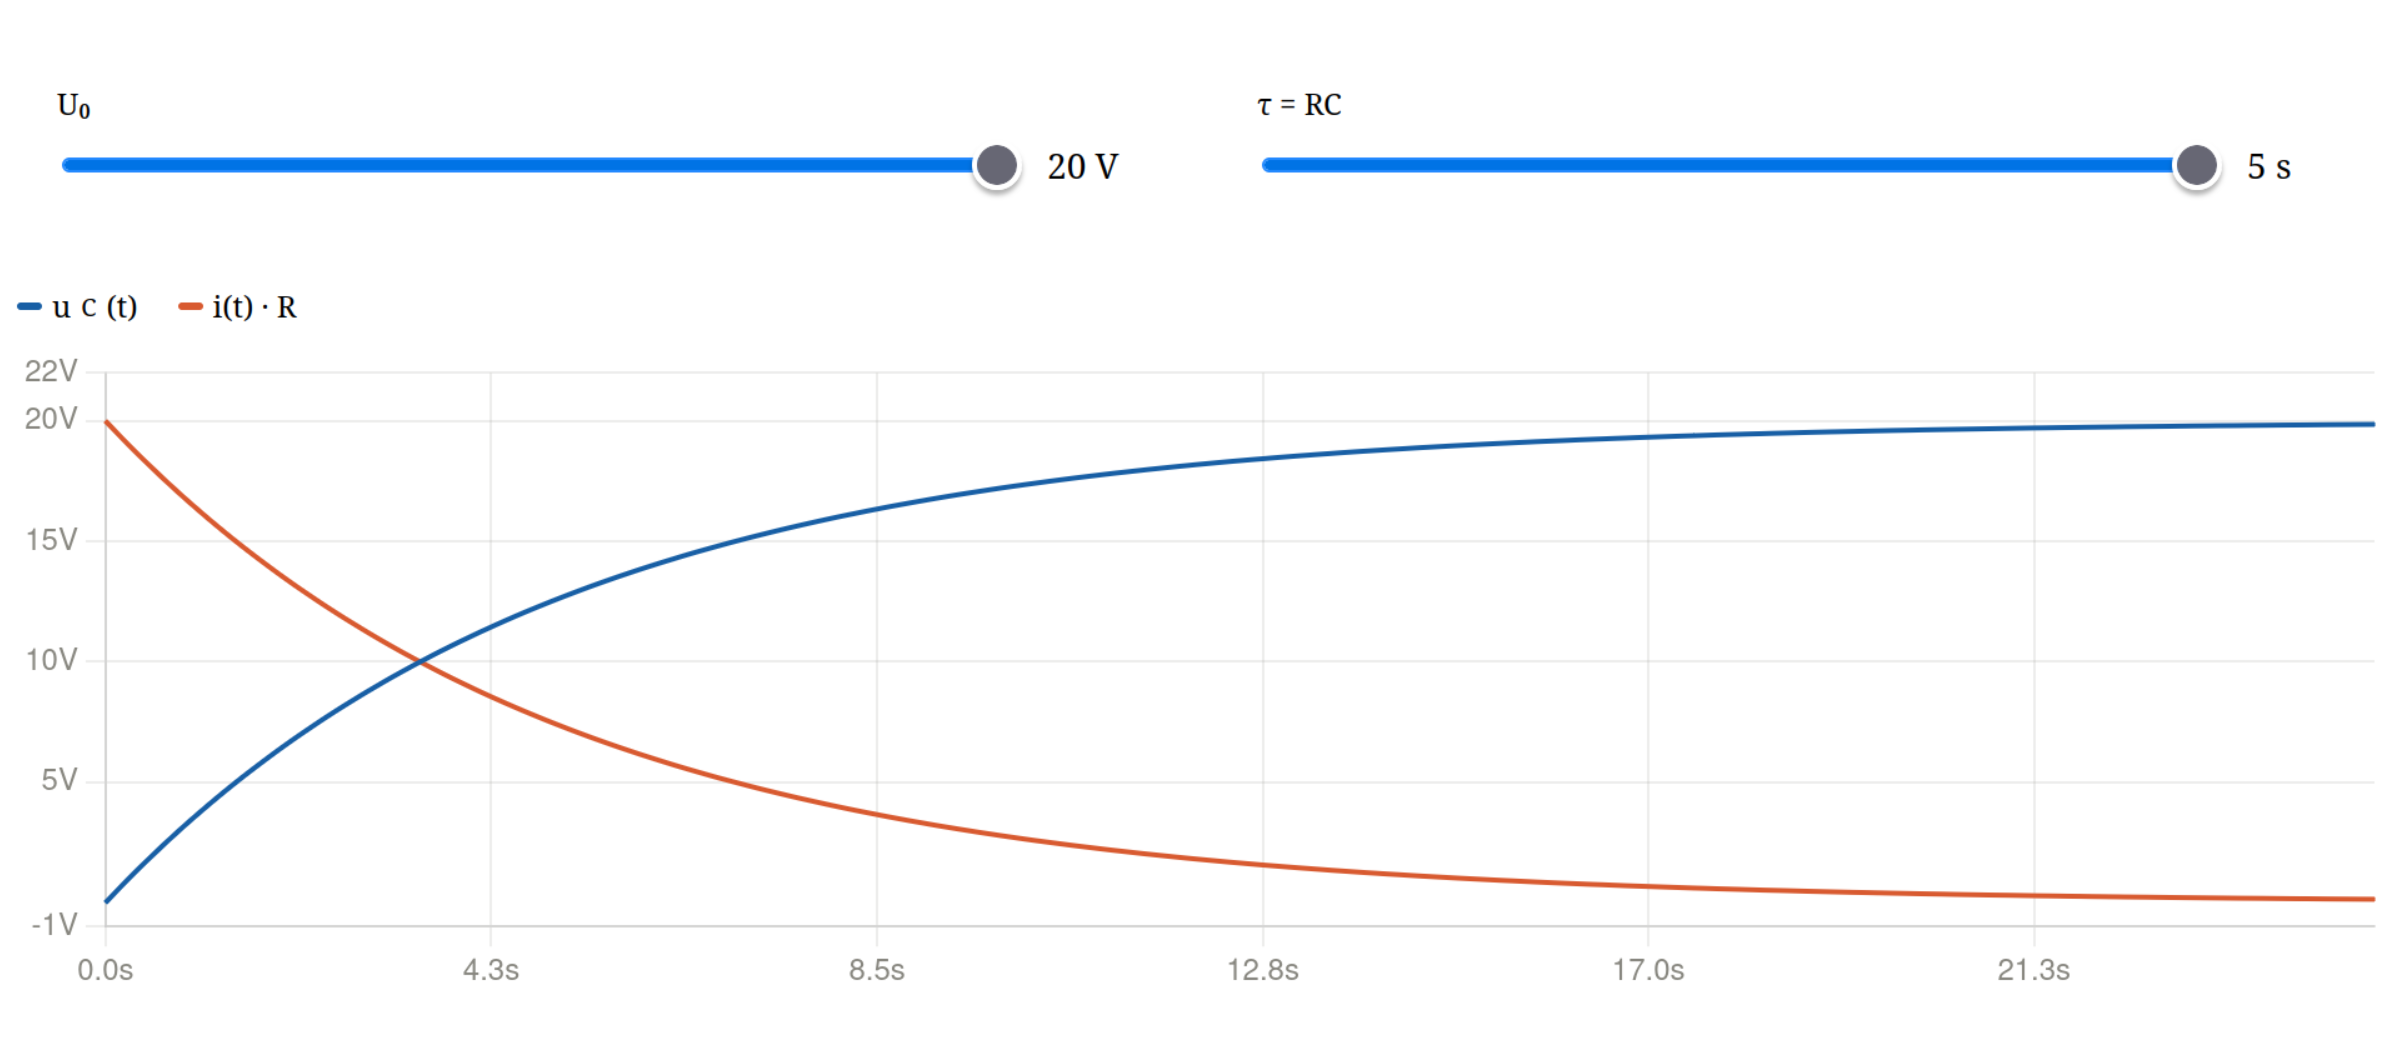
\includegraphics[width=0.5\textwidth]{img/spule_entladen} \\
	\end{tabular}
	
	\subsection{Zeitkonstanten beim Laden und Entladen einer Spule}
	
	Die Zeitkonstante hängt von der \textbf{Schaltungstopologie} ab und muss 
	für jeden Schaltzustand separat bestimmt werden.
	
	\subsubsection*{Laden ($\tau_L$) -- Schalter schliesst bei $t = 0$}
	\begin{enumerate}
		\item Spule entfernen, Quellen deaktivieren
		\item $R_{\text{Th,L}}$ an den Spulenklemmen berechnen
	\end{enumerate}
	\[
	\tau_L = \frac{L}{R_{\text{Th,L}}}
	\]
	
	\subsubsection*{Entladen ($\tau_E$) -- Schalter öffnet bei $t = 0$}
	\begin{enumerate}
		\item Spule entfernen, Quellen deaktivieren
		\item $R_{\text{Th,E}}$ an den Spulenklemmen berechnen
		(neue Topologie beachten!)
	\end{enumerate}
	\[
	\tau_E = \frac{L}{R_{\text{Th,E}}}
	\]
	
	\noindent Im Allgemeinen gilt $\tau_L \neq \tau_E$, da sich durch den 
	Schaltervorgang die Topologie und damit $R_{\text{Th}}$ ändert.\\
	\\
	\noindent Um den Thévenin-Ersatzwiderstand zu bestimmen, werden alle 
	unabhängigen Quellen deaktiviert:
	
	\begin{tabular}{l l}
		\hline
		\textbf{Quelle} & \textbf{Deaktiviert} \\
		\hline
		Spannungsquelle & Kurzschluss \\
		Stromquelle     & Offener Schalter \\
		\hline
	\end{tabular}
	
	\noindent Schalter bleiben in ihrem jeweiligen Schaltzustand.
	
	\subsection{Schaltvorgänge von Spulen}
	
	\begin{tabular}{p{0.45\textwidth} p{0.45\textwidth}}
		\vspace{0pt}
		Wird eine Spule an eine Gleichspannung angeschlossen, dann fließt im Augenblick des Einschaltens wegen der hohen Gegenspannung $U_L$ kein Strom im Kreis.
		$$I_{L,max} = \frac{U}{R_{Dr}}$$
		$$U = i_L \cdot R_{Dr} + U_L$$
		&
		\vspace{0pt}
		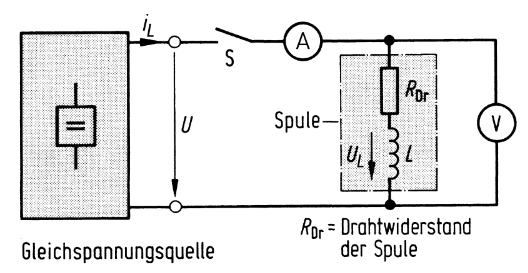
\includegraphics[width=0.5\textwidth]{img/schaltung_spule} \\
	\end{tabular}
	
	
	
	\section{Wechselspannung}
	
	\subsection{Kerngrössen von Wechselspannung und Wechselstrom}
	
	\subsection{Idealer Wirkwiderstand an Wechselspannung}
	
	\begin{tabular}{p{0.45\textwidth} p{0.45\textwidth}}
		\vspace{0pt}
		Bei einem Wirkwiderstand haben \textbf{Strom} und \textbf{Spannung} 
		immer die gleiche Phase:
		&
		\vspace{0pt}
		\includegraphics[width=0.5\textwidth]{img/wirkwiderstand} \\
	\end{tabular}
	
	\textbf{Ohmsches Gesetzt für Effektivwerte}
	$$U=R*I$$
	
	\textbf{Ohmsches Gesetzt mit Augenblickwerten}
	$$u = i * R = \hat{i} * R * sin(\omega * t)$$
	
	\subsection{Idealer Kondensator an Wechselspannung}
	
	\begin{tabular}{p{0.45\textwidth} p{0.45\textwidth}}
		\vspace{0pt}
		Die Kondensatorspannung wirkt als Gegenspannug strombegrenzend. Die strombegrenzende Wirkung eines Kondensators im Wechselstromkreis wird als \textbf{Blindwiderstand} bezeichnet. 
		$$X_C = \text{kapazitiver Blindwiderstand}$$
		$$X_C = \frac{U_c}{I_c}$$
		$$[X_C] = \Omega$$
		&
		\vspace{0pt}
		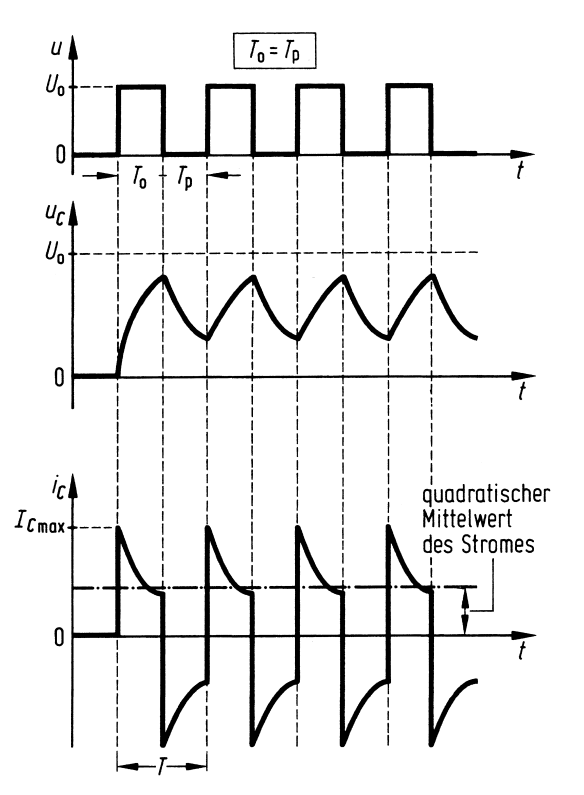
\includegraphics[width=0.5\textwidth]{img/kondensator_wechselfrequenz} \\
		
		\vspace{0pt}
		Der kapazitive Blindwiderstand wird durch din Kapaiztätwert und die Frequenz der angelegten Wechselspannung bestimmt. & 
		\vspace{0pt}
		$$X_C = f(C,f)$$
		$$X_C = \frac{1}{2\pi * f * C} = \frac{1}{\omega * C}$$ \\
		
		\vspace{0pt}
		Analog zum Gleichstrom existiert auch für den Wechselstrom das reziproke zum Widerstand: \textbf{kapazitiver Blindleitwert} & 
		\vspace{0pt}
		$$B_C = \frac{1}{X_C} = \frac{\omega * C}{1}$$
		$$[B_C] = \frac{1}{\Omega} = S (Siemens)$$ \\
		
		\vspace{0pt}
		Der \textbf{Strom} in einem Kondensator \textbf{eilt} der Spannung an ihm um \textbf{90° voraus}. & 
		\vspace{0pt} 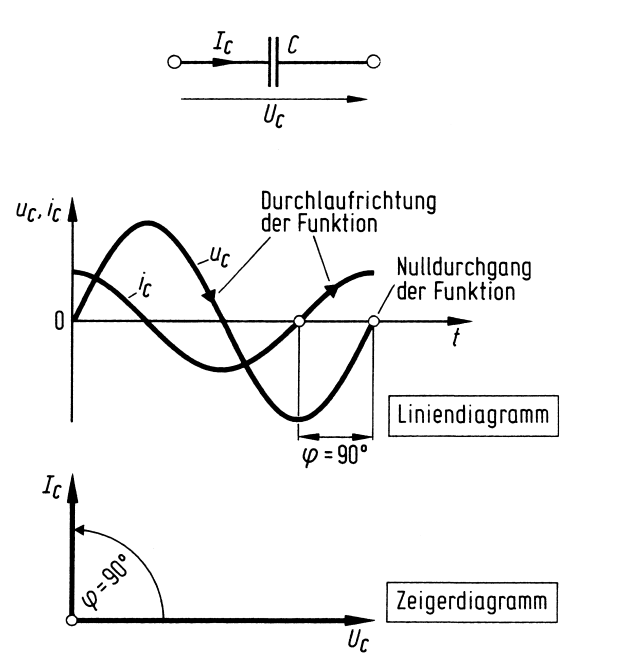
\includegraphics[width=0.5\textwidth]{img/kondensator_phasenverschiebung}
	\end{tabular}
	
	\subsection{Ideale Spule an Wechselspannung}
	
	\begin{tabular}{p{0.45\textwidth} p{0.45\textwidth}}
		\vspace{0pt}
		Die in der Spule erzeugte Gegenspannung wirk strombegrenzend. Die Spule verhält sich somit im Wechselstromkreus wie ein Widerstand. \textbf{Induktiver BLindwiderstand} = Wiederstand der Spule im Wechselstrom. 
		
		&
		
		\vspace{0pt}
		$$X_L = \text{induktiver Blindwiderstand}$$
		$$X_L = \frac{U_L}{I_L}$$
		$$[X_L] = \Omega$$ \\
		
		\vspace{0pt}
		Der induktive Blindwiderstand wird durch die Induktivität und die Frequenz der angelegten Wechselspannung bestimmt. & 
		\vspace{0pt}
		$$X_L = f(L,f)$$
		$$X_L = 2\pi * f * L = \omega * L$$ \\
		
		\vspace{0pt}
		Analog zum Gleichstrom existiert auch für den Wechselstrom das reziproke zum Widerstand: \textbf{induktive Blindleitwert} & 
		\vspace{0pt}
		$$B_L = \frac{1}{X_L} = \omega * L$$
		$$[B_L] = \frac{1}{\Omega} = S (Siemens)$$ \\
		
		\vspace{0pt}
		Der \textbf{Strom} in einer Spule \textbf{eilt} der Spannung an ihm um \textbf{90° nach}. & 
		\vspace{0pt} 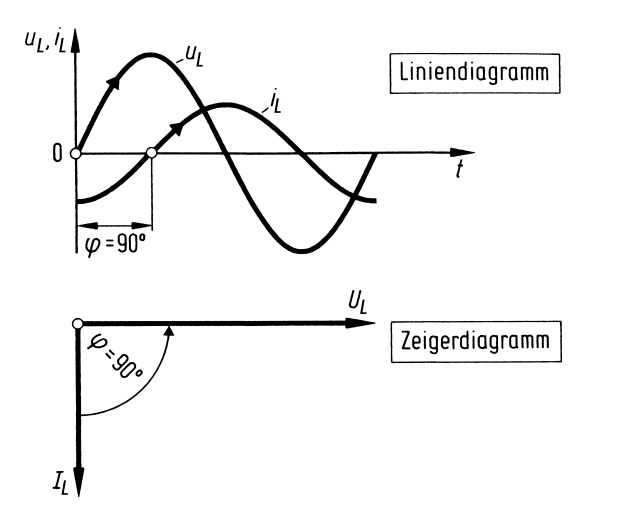
\includegraphics[width=0.5\textwidth]{img/spule_phasenverschiebung}
	\end{tabular}
	
	\subsection{Zusammenfassung: Wirkwiderstand, Kondensator und Spule}
	
	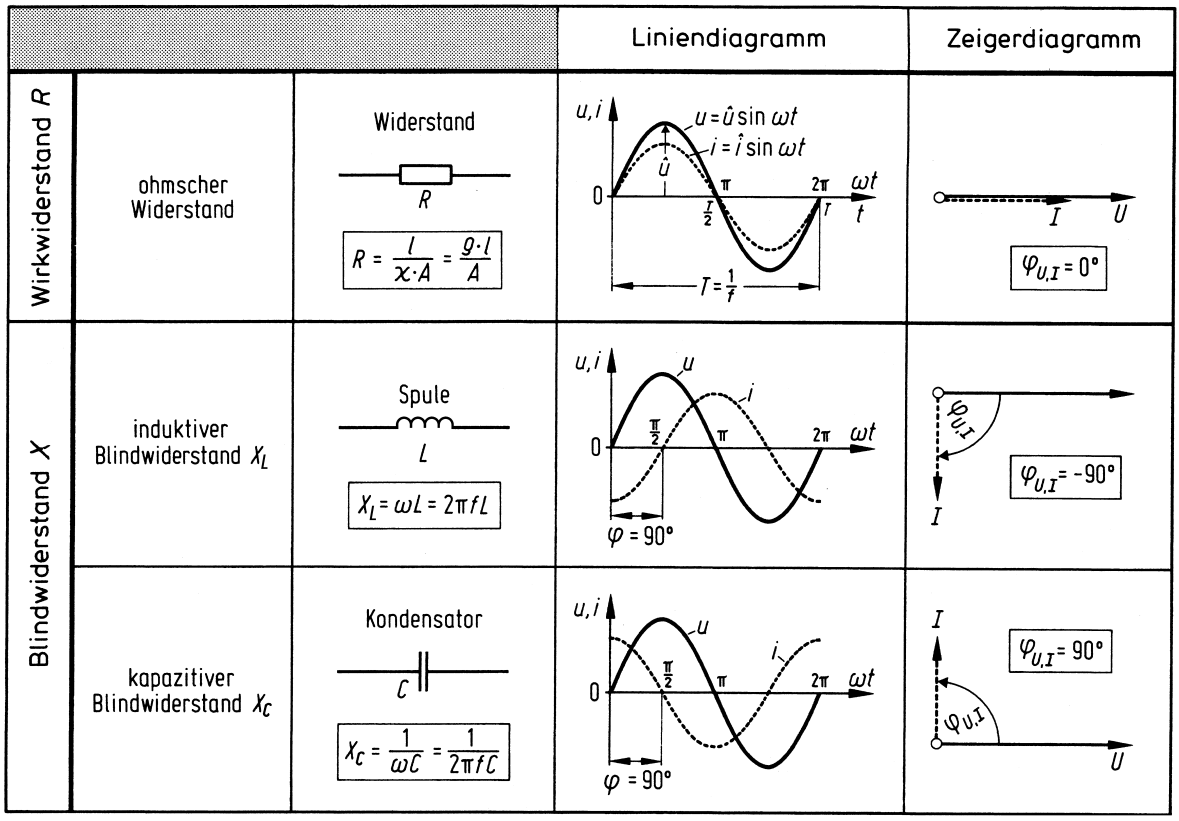
\includegraphics[width=1\textwidth]{img/zusammenfassung}
	
	\subsection{Elektrische Grössen in komplexer Schreibweise}
	
	\begin{tabular}{p{0.45\textwidth} p{0.45\textwidth}}
		\vspace{0pt}
		Da wir für den Wechselstrom zwei verschiedene Grössen verwenden, die sich durch einen Winkel unterscheiden, bietet es sich sehr an, die Grössen mit komplexen Zhaen darzustellen.
		
		&
		
		\vspace{0pt}
		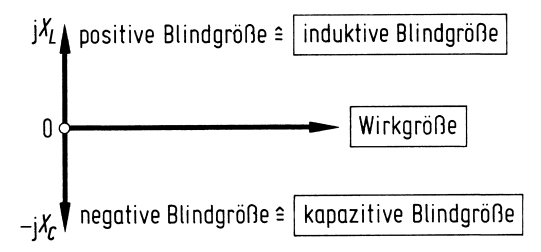
\includegraphics[width=0.5\textwidth]{img/elektrische_grössen}
		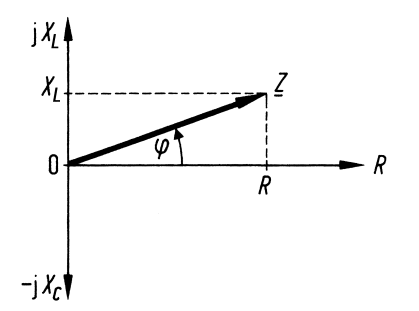
\includegraphics[width=0.5\textwidth]{img/komplexer_elektrischer_widerstand}\\
		
		\vspace{0pt}
		\textbf{Komplexer kapazitiver Blindwiderstand}
		
		&
		
		\vspace{0pt}
		$$\frac{1}{j}X_C=-jX_C=\frac{1}{j*2\pi*f*C}=X_C*e^{-j\frac{\pi}{2}}$$\\
		
		\vspace{0pt}
		\textbf{Komplexer induktiver Blindwiderstand}
		
		&
		
		\vspace{0pt}
		$$jX_L=j*2\pi*f*L=X_L*e^{j\frac{\pi}{2}}$$\\
		
		\vspace{0pt}
		\textbf{Komplexer elektrische Grössen}
		
		&
		
		\vspace{0pt}
		$$\underline{U} = \textbf{Wechselspannung (Effektivwert)}$$
		$$\underline{I} = \textbf{Wechselstromstärke (Effektivwert)}$$
		$$\underline{Z} = \textbf{Scheinwiderstand (Impedanz)}$$
		$$\underline{Y} = \textbf{Scheinleitwert (Admittanz)}$$
		$$\underline{S} = \textbf{Scheinleistung}$$\\
		
		\vspace{0pt}
		\textbf{Normalform komplexer elektrische Grössen}
		
		&
		
		\vspace{0pt}
		$$\underline{U} = U_R \pm jU_{L,C}$$
		$$\underline{I} = I_R \pm jI_{L,C}$$
		$$\underline{Z} = R \pm jX_{L,C}$$
		$$\underline{Y} = G \pm jB_{L,C}$$
		$$\underline{S} = P \pm jQ_{L,C}$$\\
		
	\end{tabular}
	
	\subsection{Wechselstromschaltungen}
	
	\subsubsection{Serienschaltung - Widerstand und Kondensator - RC}
	
	\begin{tabular}{p{0.45\textwidth} p{0.45\textwidth}}
		\vspace{0pt}
		Schliesst man eine Reihenschaltung aus Wirkwiderstand und Kondensator an eine Wechselspannung, können aufgrund der \textbf{Phasenverschiebung} von Strom und Spannung die Widerstandwerte nicht einfach zusammengezählt werden. Hier ist es nun Sinnvoll denn Wiederstand als Komplexe zahl anzuschauen mit einem \textbf{Realteil(Wirkwiderstand)} und einem \textbf{Imagniärteil(Blindwiderstand)}. Damit lässt sich nun gut rechen und mann kann die \textbf{Scheinspannung(Gesamtspannung)} einfach ermitteln indem man den \textbf{Betrag} der komplexe Zahl berechnet:
		
		$$U_{12} = \sqrt{(U_C)^2 + (U_R)^2}$$ 
		
		&
		
		\vspace{0pt}
		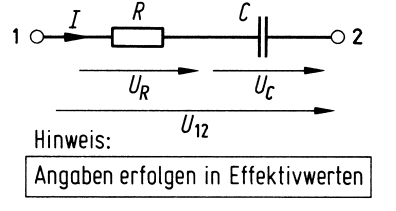
\includegraphics[width=0.5\textwidth]{img/reihenschaltung_rc}
		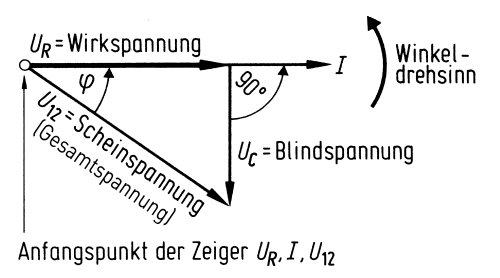
\includegraphics[width=0.5\textwidth]{img/reihenschaltung_rc_zeiger}\\
		
		\vspace{0pt}
		\textbf{Scheinwiderstand oder Impedanz}
		$$Z = \frac{U}{I}$$
		$$Z = \sqrt{R^2+(X_C)^2}$$
		$$Z = \sqrt{R^2+(\frac{1}{\omega C})^2}$$
		
		&
		\vspace{0pt}
		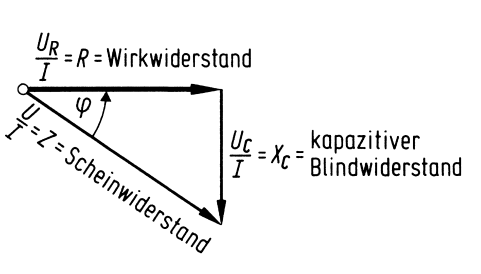
\includegraphics[width=0.5\textwidth]{img/reihenschaltung_scheinwiderstand}\\
		
		\vspace{0pt}
		In den rechtwinkligen spannungs- und Widerstanddreiecken gelten folgende Beziehungen:
		
		$$
		\sin\varphi = \frac{U_C}{U} = \frac{X_C}{Z} = \frac{\dfrac{1}{\omega C}}{\sqrt{R^2 + X_C^2}}
		$$
		
		$$
		\cos\varphi = \frac{U_R}{U} = \frac{R}{Z} = \frac{R}{\sqrt{R^2 + X_C^2}}
		$$
		
		$$
		\tan\varphi = \frac{U_C}{U_R} = \frac{X_C}{R} = \frac{\omega C}{R} = \frac{1}{\omega RC}
		$$
		
		$$
		\varphi = \arctan\frac{U_C}{U_R}
		$$
		
		&
		
		\vspace{0pt}
		In den rechtwinkligen spannungs- und Widerstanddreiecken gelten folgende Beziehungen:
		
		\vspace{0pt}
		$$
		\underline{Z} = \text{Scheinwiderstand}
		$$
		$$
		\underline{Z} = R - \mathrm{j}\, X_C = R + \frac{1}{\mathrm{j}}\, X_C = R + \frac{1}{\mathrm{j}\,\omega C}
		$$
		$$
		|\underline{Z}| = Z = \sqrt{R^2 + X_C^2}
		$$
		$$
		\underline{U} = U_R - \mathrm{j}\, U_C
		$$
		$$
		|\underline{U}| = U = \sqrt{U_R^2 + U_C^2}
		$$
		$$
		\underline{I} = \frac{\underline{U}}{\underline{Z}} = \frac{U}{Z}\,\mathrm{e}^{\mathrm{j}\,\varphi_{I,U}} = I \cdot \mathrm{e}^{\mathrm{j}\,\varphi_{I,U}}
		$$
		
		\textbf{Serieschaltung RC -- Spannungsteiler}
		$$\underline{U}_R = \underline{U} \cdot \frac{\mathrm{j}\,\omega RC}{1 + \mathrm{j}\,\omega RC}$$
		$$\underline{U}_C = \underline{U} \cdot \frac{1}{1 + \mathrm{j}\,\omega RC}$$
		
	\end{tabular}
	
	\subsubsection{Serienschaltung - Widerstand und Spule - RL}
	
	\begin{tabular}{p{0.45\textwidth} p{0.45\textwidth}}
		\vspace{0pt}
		Die Reihenschaltung von R und L ist ebenfalls
		eine Reihenschaltung eines Wirk- und eines
		Blindwiderstandes. Damit wiederholt sich der
		größte Teil der Betrachtungen, wie sie für die
		Reihenschaltung von R und C angestellt
		wurden. Es ist deshalb hier lediglich eine Zu-
		sammenfassung der Gesetzmäßigkeiten erfor-
		derlich.
		
		$$U_{12} = \sqrt{(U_L)^2 + (U_R)^2}$$ 
		
		&
		
		\vspace{0pt}
		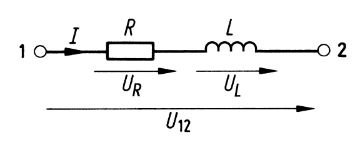
\includegraphics[width=0.5\textwidth]{img/reihenschaltung_rl}
		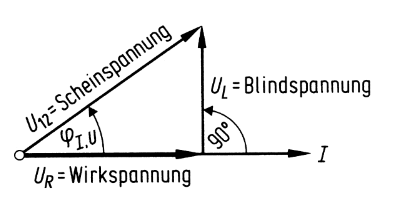
\includegraphics[width=0.5\textwidth]{img/reihenschaltung_rl_zeiger}\\
		
		\vspace{0pt}
		\textbf{Scheinwiderstand oder Impedanz}
		$$Z = \frac{U}{I}$$
		$$Z = \sqrt{R^2+{X_L}^2}$$
		$$Z = \sqrt{R^2+(\omega L)^2}$$
		
		&
		\vspace{0pt}
		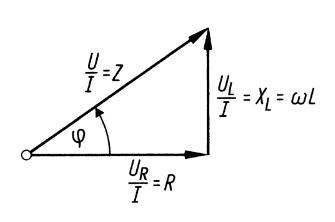
\includegraphics[width=0.5\textwidth]{img/reihenschaltung_rl_scheinwiderstand}\\
		
		\vspace{0pt}
		Aus den rechtwinkligen Zeigerdiagrammen werden die folgenden Gleichungen abgeleitet:
		
		$$\sin\varphi = \frac{U_L}{U} = \frac{X_L}{Z} = \frac{\omega L}{\sqrt{R^2 + (\omega L)^2}}$$
		
		$$\cos\varphi = \frac{U_R}{U} = \frac{R}{Z} = \frac{R}{\sqrt{R^2 + (\omega L)^2}}$$
		
		$$\tan\varphi = \frac{U_L}{U_R} = \frac{X_L}{R} = \frac{\omega L}{R}$$
		
		$$\varphi = \arctan\frac{U_L}{U_R}$$
		
		&
		
		\vspace{0pt}
		In komplexer Schreibweise ergeben sich folgende Zusammenhänge:
		
		\vspace{0pt}
		$$\underline{Z} = R + \mathrm{j}\, X_L = R + \mathrm{j}\,\omega L$$
		
		$$|\underline{Z}| = Z = \sqrt{R^2 + X_L^2}$$
		
		$$\underline{U} = U_R + \mathrm{j}\, U_L$$
		
		$$|\underline{U}| = U = \sqrt{U_R^2 + U_L^2}$$
		
		$$\underline{I} = \frac{\underline{U}}{\underline{Z}} = \frac{U}{Z}\,\mathrm{e}^{\,\mathrm{j}\varphi_{I,U}} = I \cdot \mathrm{e}^{\,\mathrm{j}\varphi_{I,U}}$$
		
		\textbf{Serieschaltung RL -- Spannungsteiler}
		$$\underline{U}_R = \underline{U} \cdot \frac{R}{R + \mathrm{j}\,\omega L}$$
		$$\underline{U}_L = \underline{U} \cdot \frac{\mathrm{j}\,\omega L}{R + \mathrm{j}\,\omega L}$$
		
	\end{tabular}
	
	\subsubsection{Serienschaltung - Kondensator und Spule - LC}
	
	\begin{tabular}{p{0.45\textwidth} p{0.45\textwidth}}
		\vspace{0pt}
		In der nun zu betrachtenden Schaltung sind
		zwei Blindgrößen in Reihe geschaltet. Die
		Spannung eilt im induktiven Blindwiderstand
		dem Strom vor, im kapazitivem Blindwider-
		stand eilt sie dagegen nach. Diese Erkenntnis-
		se werden im Zeigerdiagramm veranschau-
		licht. Aus dem Zeigerdiagramm erkennt man die
		Gegenphasigkeit der beiden Blindspannungen,
		d. h., UL und UC sind gegeneinander um 180)
		phasenverschoben. Abhängig von ihren Wer-
		ten ist somit eine teilweise oder vollständige
		Kompensation möglich. Es können \textbf{drei Fälle}
		unterschieden werden:
		
		&
		
		\vspace{0pt}
		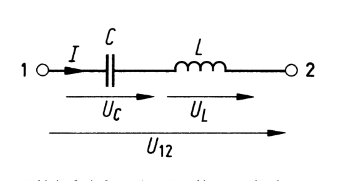
\includegraphics[width=0.4\textwidth]{img/reihenschaltung_cl}
		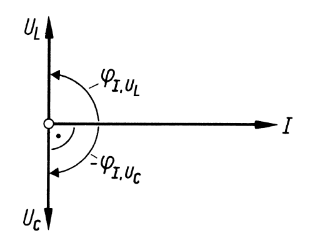
\includegraphics[width=0.4\textwidth]{img/reihenschaltung_cl_zeiger}\\
		
		\vspace{0pt}
		\textbf{1. Fall: $U_L > U_C$}\\
		Wegen der nur teilweisen Kompensation bleibt
		eine induktive Restspannung $U_{L,rest}$ bestehen.
		$$U_{L,rest} = U_L - U_C$$
		$$X_{L,rest} = \omega*L - \frac{1}{\omega*C}=\omega*L'$$
		
		\textbf{$L'$ = verbleibende wirksame Induktivität}
		&
		\vspace{0pt}
		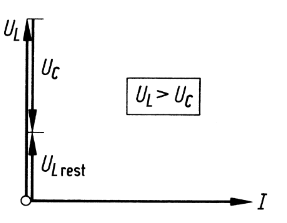
\includegraphics[width=0.4\textwidth]{img/reihenschaltung_cl_1fall}\\
		
		\vspace{0pt}
		\textbf{2. Fall: $U_L < U_C$}\\
		Hier bleibt eine kapazitive Restspannung $U_C,rest$ bestehen.
		$$U_{C,rest} = U_C - U_L$$
		$$X_{C,rest} = X_C-X_L = \frac{1}{\omega*C'}$$
		
		\textbf{$C'$ = verbleibende wirksame Kapazität}
		&
		\vspace{0pt}
		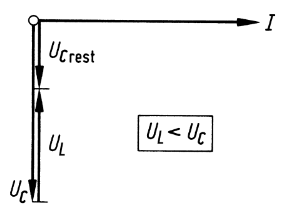
\includegraphics[width=0.4\textwidth]{img/reihenschaltung_cl_2fall}\\
		
		\vspace{0pt}
		\textbf{3. Fall: $U_L = U_C$}\\
		Die beiden Blindspannungen heben sich voll-
		ständig auf. Dieser Sonderfall wird als \textbf{Resonanzfall} definiert
		
		&
		
		\vspace{0pt}
	\end{tabular}
	
	\subsubsection{Serienschaltung - Widerstand, Kondensator und Spule - RLC}
	
	\begin{tabular}{p{0.45\textwidth} p{0.45\textwidth}}
		\vspace{0pt}
		Man beginnt Berechnungen im Wechselstrom-
		kreis in der Regel mit der Darstellung des all-
		gemeinen Zeigerdiagrammes der Spannungen
		und Ströme. Im vorliegenden Falle wird von
		UL > UC ausgegangen. Es wären aber auch
		die anderen beiden Beziehungen der Blind-
		spannungen zueinander möglich.
		Für die Differenz $U_L - U_C$
		sind Fallunterscheidungen nicht erforderlich,
		da sich wegen der Quadrierung stets nur posi-
		tive Werte ergeben:
		
		$$U_{12} = \sqrt{(U_L-U_C)^2 + (U_R)^2}$$ 
		
		&
		
		\vspace{0pt}
		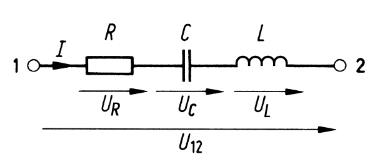
\includegraphics[width=0.4\textwidth]{img/reihenschaltung_rlc}
		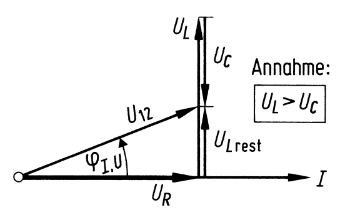
\includegraphics[width=0.4\textwidth]{img/reihenschaltung_rlc_zeiger}\\
		
		\vspace{35pt}
		\textbf{Komplexe Schreibweise Scheinspannung}\\
		$$U_{L,rest} = U_R + jU_L - jU_C$$
		
		&
		\vspace{0pt}
		\\
		
		\vspace{25pt}
		\textbf{Scheinwiderstand Z}\\
		
		$$\underline{Z} = R + \mathrm{j}\,\omega L - \mathrm{j}\,\frac{1}{\omega C}$$
		
		$$\underline{Z} = R + \mathrm{j}\left(\omega L - \frac{1}{\omega C}\right)$$
		
		$$\underline{Z} = R + \mathrm{j}\,(X_L - X_C)$$
		
		&
		\vspace{0pt}
		\\
		
		\vspace{25pt}
		\textbf{Betrag und Phasenwinkel}\\
		
		$$|\underline{Z}| = Z = \sqrt{R^2 + (X_L - X_C)^2}$$
		
		$$\varphi = \arctan\frac{X_L - X_C}{R}$$
		
		&
		
		\vspace{0pt}
		\\
	\end{tabular}
	
	\subsubsection{Parallelschaltung - Widerstand und Kondensator - RC}
	
	\begin{tabular}{p{0.45\textwidth} p{0.45\textwidth}}
		\vspace{0pt}
		Während bei einer Reihenschaltung stets die
		Stromstärke als Bezugsgröße gilt, ist dies bei
		einer Parallelschaltung die Spannung, da sie
		für alle parallel liegenden Widerstände gleich
		ist. Der Strom I teilt sich dagegen in der gege-
		benen Schaltung in einen Wirkstrom $I_R$ und
		einen Blindstrom $I_C$ auf.
		
		\textbf{Scheinstrom (Gesamtstrom)}
		$$I = \sqrt{I_R^2 + I_C^2}$$
		$$I_R = \frac{U_{12}}{R}$$
		$$I_C = \frac{U_{12}}{X_C}$$
		
		&
		
		\vspace{0pt}
		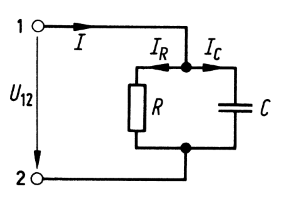
\includegraphics[width=0.4\textwidth]{img/parallelschaltung_rc}
		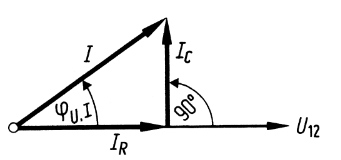
\includegraphics[width=0.4\textwidth]{img/parallelschaltung_rc_zeiger}\\
		
		\vspace{35pt}
		\textbf{Scheinleitwert }
		$$Y = \sqrt{\frac{1}{R^2}+\frac{1}{X_C^2}}=\sqrt{G^2+B_C^2}$$
		Aus dem Stromzeigerdiagramm entsteht bei
		Division aller Seiten durch U12 das Leitwert-
		zeigerdiagramm.
		
		&
		\vspace{0pt}
		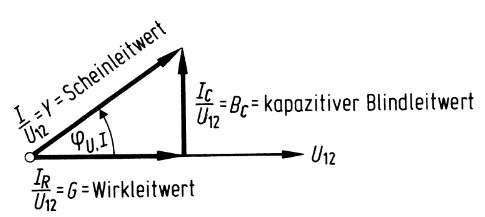
\includegraphics[width=0.4\textwidth]{img/parallelschaltung_rc_zeiger_leitwert}\\
		
		\vspace{25pt}
		\textbf{Ersatzscheniwiederstand}
		
		$Z_{\mathrm{E}}$ = \textbf{Ersatzscheinwiderstand}
		
		$$Z_{\mathrm{E}} = \frac{1}{Y} = \frac{1}{\sqrt{G^2 + B_C^2}}$$
		
		$$Z_{\mathrm{E}} = \frac{R \cdot X_C}{\sqrt{R^2 + X_C^2}}$$
		
		&
		
		\vspace{25pt}
		\textbf{Phasenwinkel}
		
		\vspace{0pt}
		$$\cos\varphi = \frac{I_R}{I} = \frac{G}{Y}$$
		
		$$\sin\varphi = \frac{I_C}{I} = \frac{B_C}{Y}$$
		
		$$\tan\varphi = \frac{I_C}{I_R} = \frac{B_C}{G}$$
		
		$$\varphi = \arctan\frac{B_C}{G}$$
		\\
		
		\vspace{5pt}
		\textbf{Scheinleitwert - Komplex}
		
		$$\underline{Y} = G + \mathrm{j}\,B_C$$
		
		$$|\underline{Y}| = Y = \sqrt{G^2 + B_C^2}$$
		
		&
		
		\vspace{5pt}
		\textbf{Ersatzscheniwiederstand - Komplex}
		
		\vspace{0pt}
		$$\underline{Z}_{\mathrm{E}} = \underbrace{\frac{R \cdot X_C^2}{R^2 + X_C^2}}_{\text{Realteil}} - \mathrm{j}\underbrace{\frac{R^2 \cdot X_C}{R^2 + X_C^2}}_{\text{Imaginärteil}}$$
		\\
		
		\textbf{Parallelschaltung RC -- Stromteiler}
		$$\underline{I}_R = \underline{I} \cdot \frac{1}{1 + \mathrm{j}\,\omega RC}$$
		$$\underline{I}_C = \underline{I} \cdot \frac{\mathrm{j}\,\omega RC}{1 + \mathrm{j}\,\omega RC}$$
		
	\end{tabular}
	
	\subsubsection{Parallelschaltung - Widerstand und Kondensator - RL}
	
	\begin{tabular}{p{0.45\textwidth} p{0.45\textwidth}}
		\vspace{0pt}
		Während bei einer Reihenschaltung stets die
		Stromstärke als Bezugsgröße gilt, ist dies bei
		einer Parallelschaltung die Spannung, da sie
		für alle parallel liegenden Widerstände gleich
		ist. Der Strom I teilt sich dagegen in der gege-
		benen Schaltung in einen Wirkstrom $I_R$ und
		einen Blindstrom $I_C$ auf.
		
		\textbf{Scheinstrom (Gesamtstrom)}
		$$I = \sqrt{I_R^2 + I_L^2}$$
		$$I_R = \frac{U_{12}}{R}$$
		$$I_C = \frac{U_{12}}{X_L}$$
		
		&
		
		\vspace{0pt}
		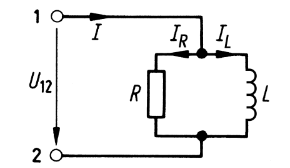
\includegraphics[width=0.4\textwidth]{img/parallelschaltung_rl}
		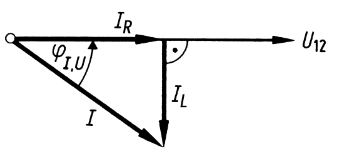
\includegraphics[width=0.4\textwidth]{img/parallelschaltung_rl_zeiger}\\
		
		\vspace{35pt}
		\textbf{Scheinleitwert }
		$$Y = \sqrt{\frac{1}{R^2}+\frac{1}{X_L^2}}=\sqrt{G^2+B_L^2}$$
		Aus dem Stromzeigerdiagramm entsteht bei
		Division aller Seiten durch U12 das Leitwert-
		zeigerdiagramm.
		
		&
		\vspace{0pt}
		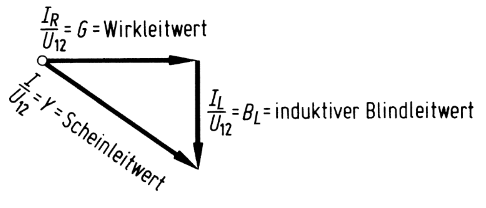
\includegraphics[width=0.4\textwidth]{img/parallelschaltung_rl_zeiger_leitwert}\\
		
		\vspace{25pt}
		\textbf{Ersatzscheniwiederstand}
		
		$Z_{\mathrm{E}}$ = \textbf{Ersatzscheinwiderstand}
		
		$$Z_{\mathrm{E}} = \frac{1}{Y} = \frac{1}{\sqrt{G^2 + B_L^2}}$$
		
		$$Z_{\mathrm{E}} = \frac{R \cdot X_L}{\sqrt{R^2 + X_L^2}}$$
		
		&
		
		\vspace{25pt}
		\textbf{Phasenwinkel}
		
		\vspace{0pt}
		$$\cos\varphi = \frac{I_R}{I} = \frac{G}{Y}$$
		
		$$\sin\varphi = \frac{I_L}{I} = \frac{B_L}{Y}$$
		
		$$\tan\varphi = \frac{I_L}{I_R} = \frac{B_L}{G}$$
		
		$$\varphi = \arctan\frac{B_L}{G}$$
		\\
		
		\vspace{5pt}
		\textbf{Scheinleitwert - Komplex}
		
		$$\underline{Y} = G + \mathrm{j}\,B_L$$
		
		$$|\underline{Y}| = Y = \sqrt{G^2 + B_L^2}$$
		
		&
		
		\vspace{5pt}
		\textbf{Ersatzscheniwiederstand - Komplex}
		
		\vspace{0pt}
		$$\underline{Z}_{\mathrm{E}} = \underbrace{\frac{R \cdot X_L^2}{R^2 + X_L^2}}_{\text{Realteil}} - \mathrm{j}\underbrace{\frac{R^2 \cdot X_L}{R^2 + X_L^2}}_{\text{Imaginärteil}}$$
		\\
		
		\textbf{Parallelschaltung RL -- Stromteiler}
		$$\underline{I}_R = \underline{I} \cdot \frac{\mathrm{j}\,\omega L}{R + \mathrm{j}\,\omega L}$$
		$$\underline{I}_L = \underline{I} \cdot \frac{R}{R + \mathrm{j}\,\omega L}$$
		
	\end{tabular}
	
	\subsubsection{Parallelschaltung - Kondensator und Spule - LC}
	
	\begin{tabular}{p{0.45\textwidth} p{0.45\textwidth}}
		\vspace{0pt}
		Die Parallelschaltung von L und C besteht nur
		aus Blindwiderständen. Beide Ströme sind ge-
		genüber der Versorgungsspannung jeweils um
		90) phasenverschoben, und zwar eilt IC um
		90) vor, während IL um 90) nacheilt. Somit
		sind die beiden Ströme zueinander gegenpha-
		sig und heben sich je nach Größe ganz oder
		teilweise auf. Es lassen sich folgende Fälle
		unterscheiden.
		
		&
		
		\vspace{0pt}
		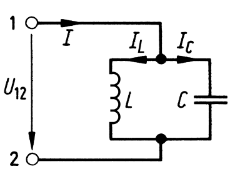
\includegraphics[width=0.4\textwidth]{img/parallelschaltung_lc}
		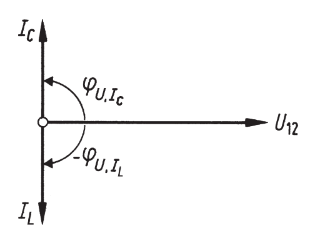
\includegraphics[width=0.4\textwidth]{img/parallelschaltung_lc_zeiger}\\
		
		\vspace{0pt}
		\textbf{1. Fall: $I_L > I_C$}\\
		Es verbleibt ein induktiver Reststrom $I_{L,rest}$
		$$I_{L\,\mathrm{rest}} = I_L - I_C$$
		
		$$X_{L\,\mathrm{rest}} = \frac{X_L \cdot X_C}{X_L - X_C}$$
		
		\textbf{$L'$ = verbleibende wirksame Induktivität}
		&
		\vspace{0pt}
		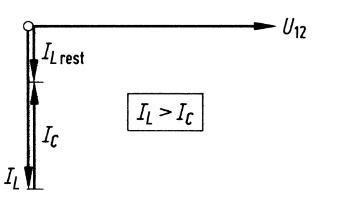
\includegraphics[width=0.4\textwidth]{img/parallelschaltung_lc_1fall}\\
		
		\vspace{0pt}
		\textbf{2. Fall: $I_L < I_C$}\\
		Es verbleibt ein kapazitiver Reststrom $I_{C,rest}$ :
		$$I_{C\,\mathrm{rest}} = I_C - I_L$$
		
		$$X_{C\,\mathrm{rest}} = \frac{X_C \cdot X_L}{X_C - X_L}$$
		
		\textbf{$C'$ = verbleibende wirksame Kapazität}
		&
		\vspace{0pt}
		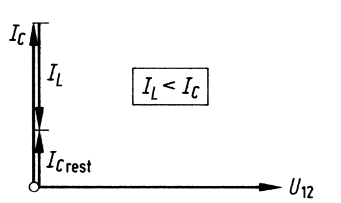
\includegraphics[width=0.4\textwidth]{img/parallelschaltung_lc_2fall}\\
		
		\vspace{0pt}
		\textbf{3. Fall: $I_L = I_C$}\\
		Die beiden Blindströme heben sich voll-
		ständig auf. Dieser Sonderfall wird als \textbf{Resonanzfall} definiert
		
		&
		
		\vspace{0pt}
	\end{tabular}
	
	\subsubsection{Parallelschaltung - Widerstand, Kondensator und Spule - RLC}
	
	\begin{tabular}{p{0.45\textwidth} p{0.45\textwidth}}
		\vspace{0pt}
		Die Betrachtung einer Parallelschaltung von
		$R, L$ und $C$ kann sich auf die bisherigen Er-
		kentnisse stützen. Als Überblick dient wiederum das allgemeine Stromzeigerdiagramm. Es
		wird angenommen, dass $X_L > X_C$ ist, also der
		Fall $I_L < I_C$ vorliegt.
		$$I = \sqrt{I_R^2 + (I_C - I_L)^2}$$
		&
		
		\vspace{0pt}
		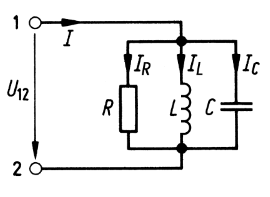
\includegraphics[width=0.4\textwidth]{img/parallelschaltung_rlc}
		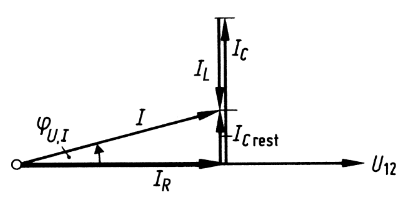
\includegraphics[width=0.4\textwidth]{img/parallelschaltung_rlc_zeiger}\\
		
		\vspace{35pt}
		\textbf{Komplexe Schreibweise Scheinstrom}\\
		$$\underline{I} = I_R + \mathrm{j}\,I_C - \mathrm{j}\,I_L$$
		
		$$\underline{I} = I_R + \mathrm{j}\,(I_C - I_L)$$
		
		&
		\vspace{0pt}
		\\
		
		\vspace{25pt}
		\textbf{Komplexe schreibweise Scheinleitwert}\\
		
		$$\underline{Y} = \frac{1}{R} + \mathrm{j}\left(\frac{1}{X_C} - \frac{1}{X_L}\right)$$
		
		$$\text{mit} \quad \frac{1}{R} = G; \quad \frac{1}{X_C} = B_C; \quad \frac{1}{X_L} = B_L$$
		
		$$\underline{Y} = G + \mathrm{j}\,(B_C - B_L)$$
		
		&
		\vspace{0pt}
		\\
		
		\vspace{25pt}
		\textbf{Phasenwinkel}\\
		
		$$\varphi_{U,I} = \arctan\frac{B_C - B_L}{G}$$
		
		$$\varphi_{U,I} = \arctan\frac{I_C - I_L}{I_R}$$
		
		&
		
		\vspace{0pt}
		\\
		
	\end{tabular}
	
	\subsection*{Komplexer Spannungs- und Stromteiler}
	\textbf{Spannungteiler}
	$$\underline{U}_2 = \underline{U}_1 \cdot \frac{\underline{Z}_2}{\underline{Z}_1 + \underline{Z}_2}$$
	
	\textbf{Stromteiler}
	$$\underline{I}_2 = \underline{I} \cdot \frac{\underline{Z}_1}{\underline{Z}_1 + \underline{Z}_2}$$
	
	
	
	\subsection*{Zusammenfassung Fachbegriffe und Formelzeichen}
	
	\textbf{Widerstände und Leitwerte:}
	\begin{tabbing}
		\hspace{1.5cm} \= \kill
		$R$ \> $=$ Wirkwiderstand $=$ Resistanz \\
		$G$ \> $=$ Wirkleitwert $=$ Konduktanz \\
		$X$ \> $=$ Blindwiderstand $=$ Reaktanz \\
		\> $X_C =$ kapazitiver Blindwiderstand $=$ Kapazitanz \\
		\> $X_L =$ induktiver Blindwiderstand $=$ Induktanz \\
		$B$ \> $=$ Blindleitwert $=$ Suszeptanz \\
		\> $B_C =$ kapazitive Suszeptanz \\
		\> $B_L =$ induktive Suszeptanz \\
		$Z$ \> $=$ Scheinwiderstand $=$ Impedanz \\
		$Y$ \> $=$ Scheinleitwert $=$ Admittanz \\
	\end{tabbing}
	
	\textbf{Komplexe elektrische Größen:}
	\begin{tabbing}
		\hspace{1.5cm} \= \kill
		$\underline{U}$ \> $=$ Wechselspannung (Effektivwert) \\
		$\underline{I}$ \> $=$ Wechselstromstärke (Effektivwert) \\
		$\underline{Z}$ \> $=$ Scheinwiderstand (Impedanz) \\
		$\underline{Y}$ \> $=$ Scheinleitwert (Admittanz) \\
		$\underline{S}$ \> $=$ Scheinleistung \\
	\end{tabbing}
	
	\section{Resonanz}
	
	\subsection{Grundlagen}
	
	\begin{tabular}{p{0.45\textwidth} p{0.45\textwidth}}
		\vspace{0pt}
		\textbf{Resonanzfall}: Die Blindwiderstände sind gleich gross und heben sich auf.
		$$X_L = X_C$$
		
		\textbf{Resonanzfrequenz}
		$$f_0 = \frac{1}{2\pi\sqrt{LC}}$$
		&
		\vspace{0pt} \\
	\end{tabular}
	
	\subsection{Idealer Serieschwingkreis (Reihenresonanzkreis)}
	
	\begin{tabular}{p{0.45\textwidth} p{0.45\textwidth}}
		\vspace{0pt}
		Im Resonanzfall fliesst ein Kurzschlussstrom: $I(f_0) \rightarrow \infty$.
		
		\textbf{Kennwiderstand}
		$$Z_0 = 2\pi f_0 L = \frac{1}{2\pi f_0 C} = \sqrt{\frac{L}{C}}$$
		
		Im Resonanzfall ist die Gesamtspannung null, aber die Blindspannungen haben definierte Werte:
		$$U_C = U_L = I(f_0) \cdot Z_0$$
		&
		\vspace{0pt}
		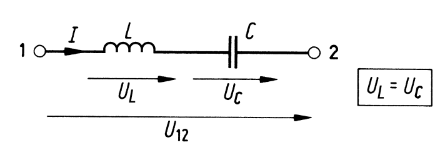
\includegraphics[width=0.45\textwidth]{img/serienschwingkreis}
		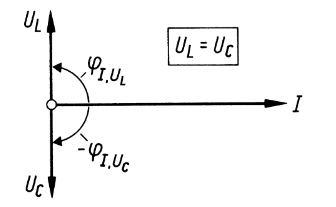
\includegraphics[width=0.45\textwidth]{img/serienschwingkreis_zeiger} \\
	\end{tabular}
	
	\subsection{Realer Serieschwingkreis (gedämpfter Reihenresonanzkreis)}
	
	\begin{tabular}{p{0.45\textwidth} p{0.45\textwidth}}
		\vspace{0pt}
		Ein realer Reihenresonanzkreis enthält neben $L$ und $C$ auch einen Ersatzwiderstand $R$. Im Resonanzfall heben sich die Blindspannungen auf, die Versorgungsspannung liegt vollständig an $R$ an -- es entsteht kein Kurzschluss.
		
		$$I_r = \frac{U_{12}}{R}$$
		$$U_L = U_C = I_r \cdot Z_0$$
		&
		\vspace{0pt}
		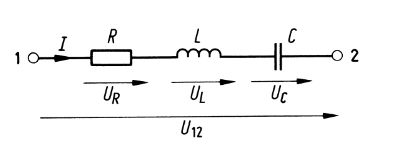
\includegraphics[width=0.45\textwidth]{img/serienschwingkreis_real}
		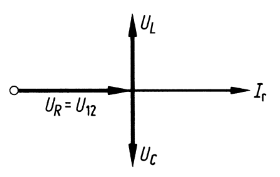
\includegraphics[width=0.45\textwidth]{img/serienschwingkreis_real_zeiger} \\
		
		\vspace{0pt}
		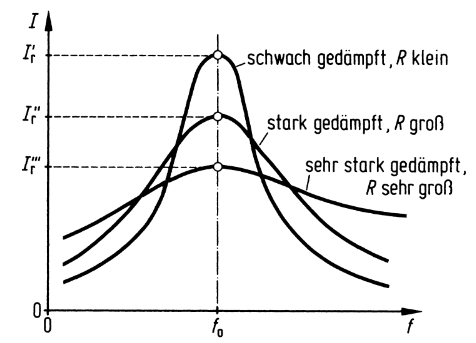
\includegraphics[width=0.5\textwidth]{img/serienschwinkreis_real_resonanzkurve}
		&
		\vspace{0pt} \\
	\end{tabular}
	
	\subsection{Idealer Parallelresonanzkreis (Sperrkreis)}
	
	\begin{tabular}{p{0.45\textwidth} p{0.45\textwidth}}
		\vspace{0pt}
		Im idealen Parallelresonanzkreis sind beide Blindströme gegenphasig und kompensieren sich vollständig. Der Gesamtstrom ist null -- der Kreis verhält sich wie ein unendlich grosser Widerstand (Sperrkreis).
		
		$$I = |I_C - I_L| = 0$$
		$$X_r \rightarrow \infty$$
		&
		\vspace{0pt}
		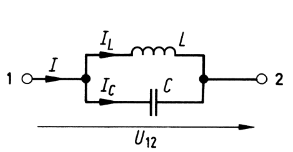
\includegraphics[width=0.45\textwidth]{img/idealer_parallelschwingkreis}
		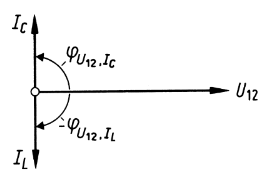
\includegraphics[width=0.45\textwidth]{img/ideale_parallelschwingkreis_zeiger} \\
		
		\vspace{0pt}
		Resonanzkurve $X = f(f)$:
		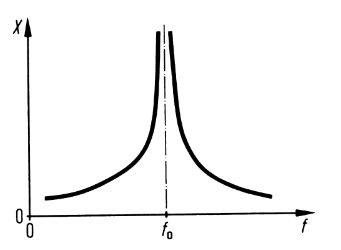
\includegraphics[width=0.5\textwidth]{img/idealer_parallelschwingkreis_resonanzkruve}
		&
		\vspace{0pt} \\
	\end{tabular}
	
	\subsection{Realer Parallelresonanzkreis (gedämpfter Parallelresonanzkreis)}
	
	\begin{tabular}{p{0.45\textwidth} p{0.45\textwidth}}
		\vspace{0pt}
		Ein realer Parallelresonanzkreis enthält einen Ersatzwiderstand $R$, der alle Wirkwiderstände zusammenfasst. Dadurch ist der Resonanzwiderstand nicht mehr unendlich gross, sondern gleich $R$ (Dämpfungswiderstand). Der Resonanzstrom $I_r$ wird entsprechend begrenzt.
		
		$$I_r = \frac{U_{12}}{R}$$
		&
		\vspace{0pt}
		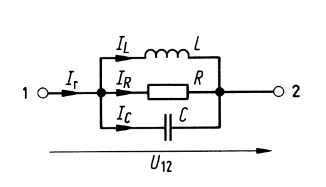
\includegraphics[width=0.45\textwidth]{img/realer_parallelschwingkreis}
		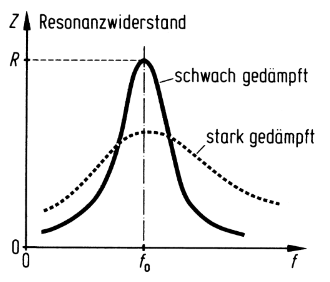
\includegraphics[width=0.45\textwidth]{img/realer_parallelschwingkreis_kurve} \\
	\end{tabular}
	
	\subsection{Resonanz-Transformator}
	
	\begin{tabular}{p{0.45\textwidth} p{0.45\textwidth}}
		\vspace{0pt}
		Parallelschaltung von $C$ mit der Serieschaltung von $R$ und $L$. Bei Resonanz erscheint am Eingang ein \textbf{anderer} Widerstand als $R$ -- daher die Bezeichnung ``Transformator''.
		
		\textbf{Admittanz der Schaltung}
		$$\underline{Y} = \frac{1}{R + j\omega L} + j\omega C = \frac{1 - \omega^2 LC + j\omega CR}{R + j\omega L}$$
		
		\textbf{Resonanzkreisfrequenz} (gültig für $L/R > RC$):
		$$\omega_r = \frac{1}{\sqrt{LC}}\sqrt{1 - \frac{RC}{L/R}}$$
		
		\textbf{Impedanz bei Resonanz} (rein reell):
		$$\underline{Z}(\omega_r) = \frac{L}{CR} \qquad \text{bzw.} \qquad \underline{Y}(\omega_r) = \frac{CR}{L}$$
		
		Bei \textbf{fixer Frequenz} kann Resonanz alternativ durch die Wahl von $R_r = \sqrt{\frac{L}{C}(1-\omega^2 LC)}$ erreicht werden.
		&
		\vspace{0pt}
		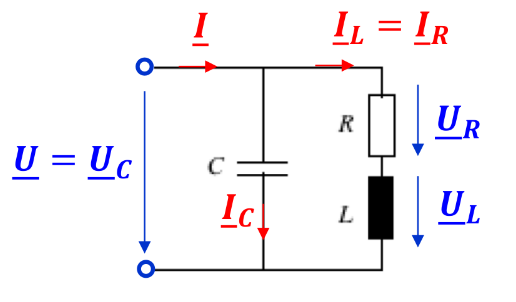
\includegraphics[width=0.45\textwidth]{img/resonanztranformator}
		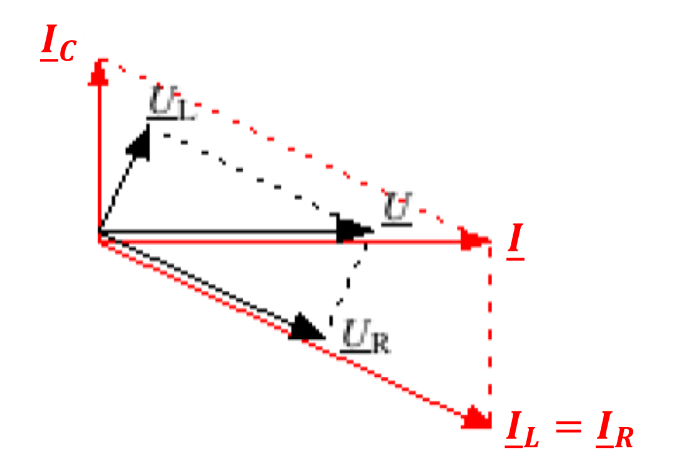
\includegraphics[width=0.45\textwidth]{img/resonanztranformator_zeiger} \\
	\end{tabular}
	
	\section{Leistung im Wechselstromkreis}
	
	\subsection{Momentanleistung}
	
	\begin{tabular}{p{0.45\textwidth} p{0.45\textwidth}}
		\vspace{0pt}
		Der zeitliche Verlauf des Energiestroms an den Klemmen eines Zweipols heisst
		\textbf{Momentanleistung}. Sie ergibt sich aus dem Produkt der Augenblickswerte:
		$$p(t) = u(t) \cdot i(t)$$
		
		Für einen linearen Zweipol bei harmonischer Anregung und
		Phasenverschiebung $\varphi = \varphi_u - \varphi_i$ gilt:
		$$p(t) = UI\cos(\varphi)\bigl[1 + \cos(2\omega t + 2\varphi_u)\bigr]
		+ UI\sin(\varphi)\sin(2\omega t + 2\varphi_u)$$
		
		Die Momentanleistung besteht aus einem \textbf{konstanten Anteil} und
		\textbf{Wechselanteilen mit doppelter Frequenz}.
		&
		\vspace{0pt}
		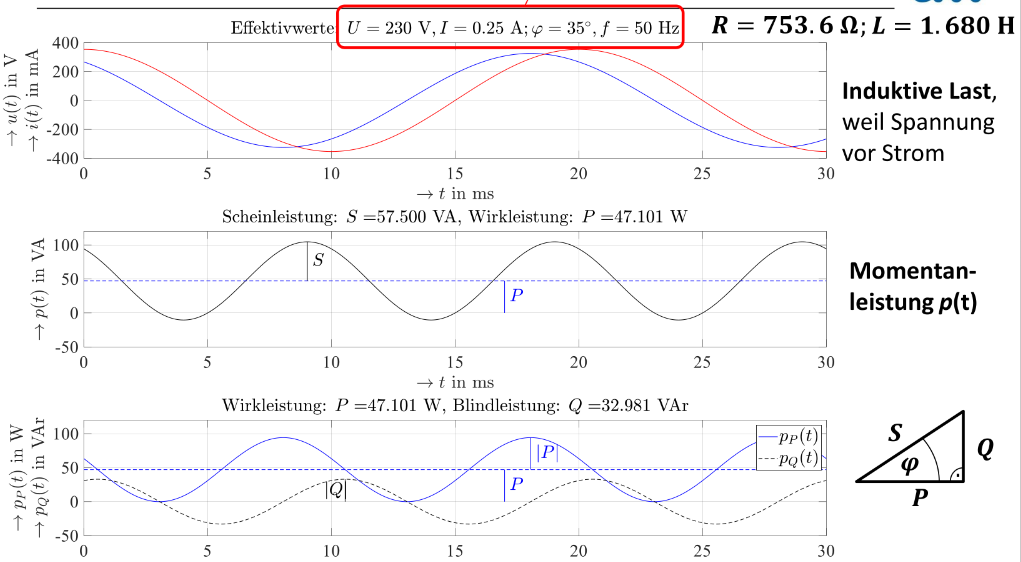
\includegraphics[width=0.5\textwidth]{img/momentanleistung_zerlegung}\\
	\end{tabular}
	
	\subsection{Wirkleistung \texorpdfstring{$P$}{P}}
	
	\begin{tabular}{p{0.45\textwidth} p{0.45\textwidth}}
		\vspace{0pt}
		Der \textbf{lineare Mittelwert} der Momentanleistung ist die \textbf{Wirkleistung}
		-- die im Mittel aufgenommene Energie pro Zeiteinheit:
		$$P = \frac{1}{T}\int_T p(t)\,\mathrm{d}t = U \cdot I \cdot \cos\varphi$$
		$$[P] = \mathrm{W \; (Watt)}$$
		
		\textbf{Interpretation:}
		\begin{itemize}[noitemsep]
			\item An einem Wirkwiderstand ist $\varphi = 0$, daher $P = U \cdot I$.
			\item An einem reinen Blindwiderstand ist $\varphi = \pm\frac{\pi}{2}$,
			daher $P = 0$ -- ein idealer Kondensator oder eine ideale Spule
			nimmt \emph{keine} Wirkleistung auf.
			\item Die auf Typenschildern angegebene Leistung ist die Wirkleistung.
		\end{itemize}
		&
		\vspace{0pt}
		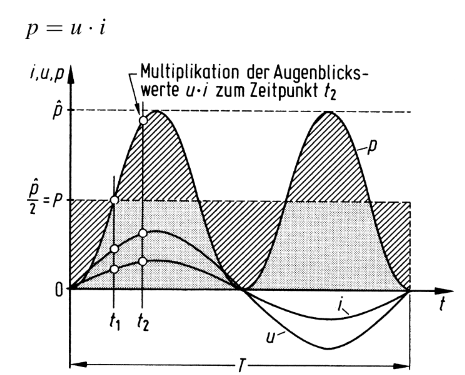
\includegraphics[width=0.5\textwidth]{img/wirkleistung_diagramm}\\
	\end{tabular}
	
	\subsection{Blindleistung \texorpdfstring{$Q$}{Q}}
	
	\begin{tabular}{p{0.45\textwidth} p{0.45\textwidth}}
		\vspace{0pt}
		Der Wechselanteil aufgrund des Blindanteils des Stromes beschreibt die
		\textbf{zwischen Quelle und Speicher pendelnde Energie}. Die Blindleistung ist:
		$$Q := U \cdot I \cdot \sin\varphi$$
		$$[Q] = \mathrm{VAr \; (Volt{-}Ampere{-}reaktiv)}$$
		
		\textbf{Vorzeichen:}
		\begin{itemize}[noitemsep]
			\item $\varphi > 0$ (Spannung eilt vor): \textbf{induktives} Verhalten,
			$Q > 0$
			\item $\varphi < 0$ (Strom eilt vor): \textbf{kapazitives} Verhalten,
			$Q < 0$
		\end{itemize}
		
		Der Blindleistungsumsatz innerhalb einer vollständigen Periode ist null -- es
		wird \emph{keine} Energie dauerhaft verbraucht, nur zwischengespeichert.
		&
		\vspace{0pt}
		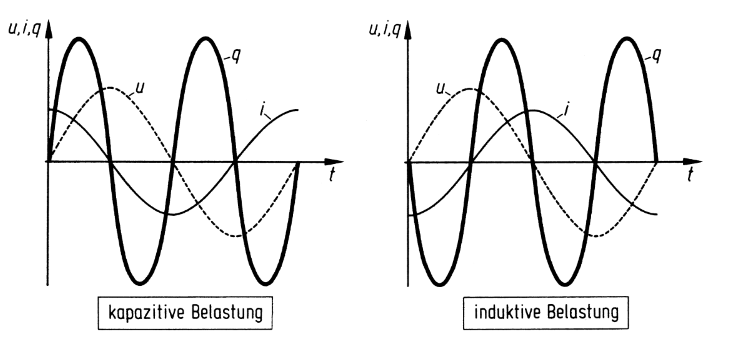
\includegraphics[width=0.5\textwidth]{img/blindleistung_diagramm}\\
	\end{tabular}
	
	\subsection{Scheinleistung \texorpdfstring{$S$}{S} und Leistungsdreieck}
	
	\begin{tabular}{p{0.45\textwidth} p{0.45\textwidth}}
		\vspace{0pt}
		Die \textbf{Amplitude des Wechselanteils} der Momentanleistung -- also das
		Produkt der Effektivwerte -- heisst \textbf{Scheinleistung}:
		$$S = U \cdot I$$
		$$[S] = \mathrm{VA \; (Volt{-}Ampere)}$$
		
		Aus dem rechtwinkligen \textbf{Leistungsdreieck} folgt:
		$$S^2 = P^2 + Q^2 \qquad S = \sqrt{P^2 + Q^2}$$
		$$P = S\cos\varphi \qquad Q = S\sin\varphi \qquad \tan\varphi = \frac{Q}{P}$$
		&
		\vspace{0pt}
		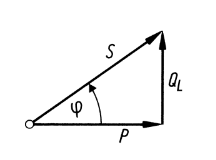
\includegraphics[width=0.5\textwidth]{img/leistungsdreieck}\\
	\end{tabular}
	
	\subsection{Komplexe Scheinleistung}
	
	\begin{tabular}{p{0.45\textwidth} p{0.45\textwidth}}
		\vspace{0pt}
		Die \textbf{komplexe Scheinleistung} fasst Wirk- und Blindleistung zusammen.
		Wichtig: Der Strom muss \textbf{konjugiert komplex} genommen werden, damit
		das Vorzeichen von $Q$ korrekt ist:
		$$\underline{S} = \underline{U} \cdot \underline{I}^* = P + jQ = S\angle\varphi$$
		
		Alternativ über Impedanz bzw. Admittanz:
		$$\underline{S} = \underline{Z} \cdot |\underline{I}|^2 = RI^2 + jXI^2$$
		$$\underline{S} = \underline{Y}^* \cdot |\underline{U}|^2 = GU^2 + j(-B)U^2$$
		
		\textbf{Achtung:} Die komplexe Scheinleistung ist \emph{kein} Zeiger für die
		Momentanleistung, da diese ein Mischsignal mit doppelter Frequenz ist.
		&
		\vspace{0pt}
		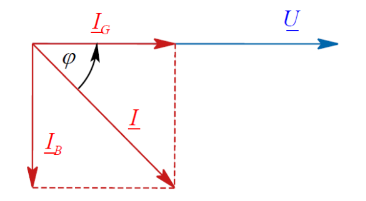
\includegraphics[width=0.5\textwidth]{img/komplexe_scheinleistung_zeiger}\\
	\end{tabular}
	
	\subsection{Leistungsfaktor}
	
	\begin{tabular}{p{0.45\textwidth} p{0.45\textwidth}}
		\vspace{0pt}
		Das Verhältnis von Wirkleistung zu Scheinleistung heisst \textbf{Leistungsfaktor}:
		$$\lambda = \cos\varphi = \frac{P}{S} = \frac{P}{U \cdot I}$$
		$$0 \leq \cos\varphi \leq 1$$
		
		Je kleiner $\cos\varphi$, desto grösser der Strom $I$ bei gleicher Wirkleistung
		$P$ und Spannung $U$. Ein kleiner Leistungsfaktor erhöht die
		Leitungsverluste unnötig.
		
		\textbf{Achtung:} Der Leistungsfaktor $\cos\varphi$ darf nicht mit dem
		Wirkungsgrad $\eta$ verwechselt werden!
		&
		\vspace{0pt}
		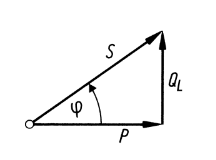
\includegraphics[width=0.5\textwidth]{img/leistungsdreieck}\\
	\end{tabular}
	
	\subsection{Blindleistungskompensation}
	
	\begin{tabular}{p{0.45\textwidth} p{0.45\textwidth}}
		\vspace{0pt}
		Typische Industrieanlagen (Motoren, Transformatoren) sind \textbf{induktiv}.
		Die dabei anfallende Blindleistung muss zwischen Erzeuger und Verbraucher
		hin- und herpendeln, was den Leitungsstrom erhöht und zu unnötigen Verlusten
		führt. Energieversorgungsunternehmen fordern daher $\cos\varphi \geq 0{,}9$.
		
		\textbf{Massnahme:} Parallelschalten eines Kondensators, der die induktive
		Blindleistung lokal liefert. Die Formel für die benötigte Kapazität bei
		vollständiger Parallelkompensation:
		$$C = \frac{Q_C}{U_N^2 \cdot 2\pi f}
		= \frac{Q_L - Q_{L,\mathrm{rest}}}{U_N^2 \cdot 2\pi f}$$
		
		mit $Q_{L,\mathrm{rest}} = P \cdot \tan\varphi'$ (Zielwinkel $\varphi'$).
		&
		\vspace{0pt}
		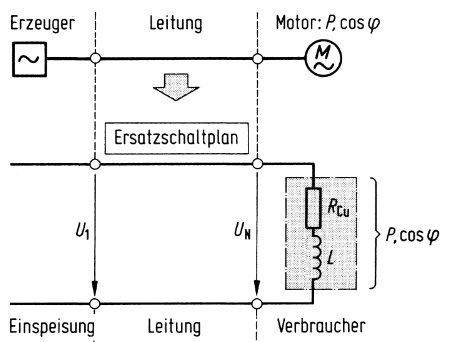
\includegraphics[width=0.5\textwidth]{img/blindleistungskompensation_schaltung}
		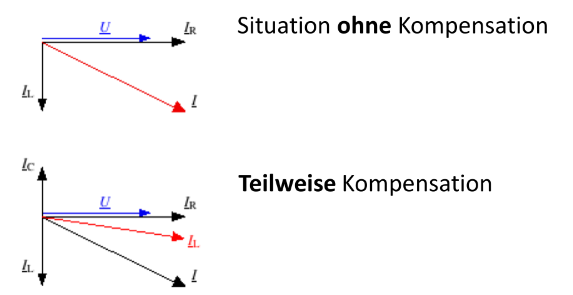
\includegraphics[width=0.5\textwidth]{img/blindleistungskompensation_zeiger}\\
		
		\vspace{0pt}
		\textbf{Strom vor und nach Kompensation:}
		$$I = \frac{P}{U_N \cdot \cos\varphi} \qquad
		I' = \frac{P}{U_N \cdot \cos\varphi'}$$
		Der neue Strom $I' < I$ entlastet die Zuleitung.
		&
		\vspace{0pt}\\
	\end{tabular}
	
	\subsection*{Zusammenfassung Leistungsgrössen}
	
	\begin{tabbing}
		\hspace{3.5cm} \= \hspace{5cm} \= \kill
		\textbf{Grösse} \> \textbf{Formel} \> \textbf{Einheit} \\[4pt]
		Wirkleistung $P$        \> $U \cdot I \cdot \cos\varphi$           \> W (Watt) \\
		Blindleistung $Q$       \> $U \cdot I \cdot \sin\varphi$           \> VAr \\
		Scheinleistung $S$      \> $U \cdot I = \sqrt{P^2+Q^2}$            \> VA \\
		Leistungsfaktor         \> $\cos\varphi = P/S$                     \> (dimensionslos) \\
		Kompl. Scheinleistung   \> $\underline{S} = \underline{U}\cdot\underline{I}^* = P+jQ$ \> VA \\
	\end{tabbing}
	
	\section{Frequenzverhalten linearer Netzwerke}
	
	% Referenz: Folie 1 (Inhaltsübersicht)
	
	% ─────────────────────────────────────────────────────────────
	\subsection{Einleitung \& Grundlagen}
	% Referenz: Folie 2–7
	% ─────────────────────────────────────────────────────────────
	
	Bei harmonischer (sinusförmiger) Anregung eines \textbf{LTI-Systems} (lineares,
	zeitinvariantes System) sind im eingeschwungenen Zustand alle Grössen ebenfalls
	harmonisch.
	
	\subsubsection*{Harmonisches Signal}
	Ein harmonisches Signal ist vollständig durch drei Parameter beschrieben:
	\begin{equation}
		x(t) = \hat{X} \cdot \cos(\omega t + \varphi_x)
	\end{equation}
	\begin{itemize}
		\item $\hat{X}$: Amplitude (Spitzenwert), Effektivwert $X = \hat{X}/\sqrt{2}$
		\item $\varphi_x$: Nullphasenwinkel
		\item $\omega = 2\pi f$: Kreisfrequenz
	\end{itemize}
	
	\subsubsection*{Komplexe Darstellung (Zeiger)}
	% Referenz: Folie 2–3
	Ein harmonisches Signal wird als komplexe Zahl (Zeiger) dargestellt:
	\begin{equation}
		\underline{X} = X \cdot e^{j\varphi_x} = X \angle \varphi_x
	\end{equation}
	Der Betrag enthält die Amplitude, das Argument die Phase.
	Die Zeitableitung entspricht im Frequenzbereich einer Multiplikation mit $j\omega$:
	\begin{equation}
		\frac{dx}{dt} \quad \longleftrightarrow \quad j\omega \cdot \underline{X}
	\end{equation}
	Dies vereinfacht Differentialgleichungen zu algebraischen Gleichungen.
	
	\subsubsection*{Fourier-Reihe \& Superposition}
	% Referenz: Folie 7
	Ein beliebiges periodisches Signal kann als Summe harmonischer Signale
	(Fourier-Reihe) dargestellt werden. Da für LTI-Systeme das
	\textbf{Superpositionsprinzip} gilt, kann die Systemantwort als Summe der
	Einzelantworten berechnet werden.
	
	% ─────────────────────────────────────────────────────────────
	\subsection{Frequenzgang -- Definitionen}
	% Referenz: Folie 8–11
	% ─────────────────────────────────────────────────────────────
	
	\subsubsection*{Frequenzgangfunktion $H(\omega)$}
	Das Verhältnis von Ausgangs- zu Eingangsgrösse als Funktion der Kreisfrequenz:
	\begin{equation}
		H(\omega) = \frac{\underline{U}_2}{\underline{U}_1}
	\end{equation}
	$H(\omega)$ ist komplex und auch bekannt als \textit{Transferfunktion} oder
	\textit{Übertragungsfunktion}.
	
	\subsubsection*{Amplitudengang und Phasengang}
	\begin{itemize}
		\item \textbf{Amplitudengang:} $|H(\omega)|$ als Funktion der Frequenz
		\item \textbf{Phasengang:} $\arg(H(\omega))$ als Funktion der Frequenz
		\item \textbf{Frequenzgang:} die Kombination beider Plots
	\end{itemize}
	Der Frequenzgang beschreibt ein LTI-System \textbf{vollständig und eindeutig}.
	
	% [BILD: Zweitor-Schema mit U1, H(omega), U2 -- Folie 10]
	
	% ─────────────────────────────────────────────────────────────
	\subsection{Normierung}
	% Referenz: Folie 24–26
	% ─────────────────────────────────────────────────────────────
	
	Um Bodediagramme unabhängig von konkreten Bauteilwerten vergleichen zu können,
	führt man die \textbf{normierte Kreisfrequenz} ein:
	\begin{equation}
		\Omega = \frac{\omega}{\omega_0}
	\end{equation}
	wobei $\omega_0$ die charakteristische Normierungsfrequenz der Schaltung ist.
	\begin{itemize}
		\item Systeme 1. Ordnung: $\omega_0 = \omega_g = \frac{1}{\tau}$
		\item Systeme 2. Ordnung (LC): $\omega_0 = \frac{1}{\sqrt{LC}}$
	\end{itemize}
	
	% ─────────────────────────────────────────────────────────────
	\subsection{Dezibel (dB)}
	% Referenz: Folie 15–17
	% ─────────────────────────────────────────────────────────────
	
	Logarithmische Darstellung von Verhältnissen (Pseudoeinheit nach A.G. Bell):
	\begin{align}
		\text{Leistungsverhältnis:} & \quad y = 10 \cdot \log_{10}\frac{P_2}{P_1} \quad [\text{dB}] \\
		\text{Spannungsverhältnis:} & \quad y = 20 \cdot \log_{10}\frac{U_2}{U_1} \quad [\text{dB}]
	\end{align}
	
	Wichtige Werte:
	\begin{center}
		\begin{tabular}{ccc}
			\hline
			dB & $U_2/U_1$ & $P_2/P_1$ \\
			\hline
			0    & 1          & 1       \\
			$-3$ & $1/\sqrt{2} \approx 0.707$ & $1/2$ \\
			$-6$ & $1/2$      & $1/4$   \\
			$-20$& $1/10$     & $1/100$ \\
			$-40$& $1/100$    & $1/10000$ \\
			\hline
		\end{tabular}
	\end{center}
	
	\subsubsection*{Absolute Pegel}
	\begin{itemize}
		\item \textbf{dBm:} Bezug $P_\text{bez} = 1\,\text{mW}$
		\item \textbf{dBV:} Bezug $U_\text{bez} = 1\,\text{V}$
		\item \textbf{dB$\mu$V:} Bezug $U_\text{bez} = 1\,\mu\text{V}$
	\end{itemize}
	
	% ─────────────────────────────────────────────────────────────
	\subsection{Systeme 1. Ordnung}
	% Referenz: Folie 12–36
	% ─────────────────────────────────────────────────────────────
	
	\subsubsection{RC-Tiefpass (1. Ordnung)}
	% Referenz: Folie 12–23
	
	% [BILD: RC-Schaltung mit U1, R, C, U2 -- Folie 12]
	
	Berechnung mit dem komplexen Spannungsteiler:
	\begin{equation}
		H(\omega) = \frac{Z_C}{Z_R + Z_C} = \frac{1}{1 + j\omega RC} = \frac{1}{1+j\omega\tau}
		\qquad \tau = RC
	\end{equation}
	Normiert mit $\Omega = \omega\tau = \omega/\omega_g$:
	\begin{equation}
		H(\Omega) = \frac{1}{1+j\Omega}
	\end{equation}
	
	\textbf{Amplitudengang:}
	\begin{equation}
		|H(\omega)| = \frac{1}{\sqrt{1+(\omega\tau)^2}}
	\end{equation}
	\textbf{Phasengang:}
	\begin{equation}
		\arg(H(\omega)) = -\arctan(\omega\tau)
	\end{equation}
	\textbf{Grenzfrequenz} (--3\,dB-Punkt):
	\begin{equation}
		\omega_g = \frac{1}{\tau} = \frac{1}{RC} \qquad f_g = \frac{1}{2\pi RC}
	\end{equation}
	Bei $\omega_g$: $|H| = 1/\sqrt{2} \approx 0.707$ (Leistung auf die Hälfte).
	
	% [BILD: Bodediagramm RC-Tiefpass, Amplitudengang + Phasengang -- Folie 18/19]
	
	\subsubsection{CR-Hochpass (1. Ordnung)}
	% Referenz: Folie 31–33
	
	% [BILD: CR-Schaltung mit U1, C, R, U2 -- Folie 31]
	
	\begin{equation}
		H(\omega) = \frac{j\omega\tau}{1+j\omega\tau} \qquad \tau = RC
	\end{equation}
	\begin{itemize}
		\item Tiefe Frequenzen: stark gedämpft
		\item Hohe Frequenzen: kaum gedämpft
		\item Bodediagramm: $+20\,\text{dB/Dekade}$ Anstieg bis $\Omega=1$
	\end{itemize}
	
	% [BILD: Bodediagramm CR-Hochpass -- Folie 32/33]
	
	\subsubsection*{Bemerkungen zu Systemen 1. Ordnung}
	% Referenz: Folie 37
	\begin{itemize}
		\item Je 1 Speicher (L oder C) und mind. 1 R
		\item Grenzfrequenz: $f_0 = \omega_0/(2\pi) = 1/(2\pi\tau)$ beim --3\,dB-Punkt
		\item LR- und RL-Schaltungen haben identische Frequenzgänge wie RC/CR
		(bei gleichem $\tau = L/R$)
	\end{itemize}
	
	% ─────────────────────────────────────────────────────────────
	\subsection{Ortskurve}
	% Referenz: Folie 27–28
	% ─────────────────────────────────────────────────────────────
	
	Parameterdarstellung von $H(\omega)$ in der komplexen Zahlenebene mit $\omega$
	als Parameter ($\omega$ von 0 bis $\infty$).
	\begin{itemize}
		\item Richtungssinn: im \textbf{Uhrzeigersinn} bei steigender Frequenz
		\item RC-Tiefpass: exakter \textbf{Halbkreis} im 4. Quadranten
		\item In der Regelungstechnik: \textit{Nyquist-Diagramm}
	\end{itemize}
	
	% [BILD: Ortskurve RC-Tiefpass, Halbkreis von (1,0) nach (0,0) -- Folie 28]
	
	Spezielle Punkte beim RC-Tiefpass:
	\begin{itemize}
		\item $\omega = 0$: $H = 1$ $\rightarrow$ Punkt $(1,\, 0)$
		\item $\omega = \omega_g$: $H = 0.5 - j0.5$ $\rightarrow$ tiefster Punkt (--3\,dB)
		\item $\omega \to \infty$: $H = 0$ $\rightarrow$ Punkt $(0,\, 0)$
	\end{itemize}
	
	% ─────────────────────────────────────────────────────────────
	\subsection{Systeme 2. Ordnung}
	% Referenz: Folie 38–62
	% ─────────────────────────────────────────────────────────────
	
	Netzwerke mit \textbf{zwei verschiedenen Speichern} (C und L) und mind. 1 R.
	
	\subsubsection{LRC-Tiefpass (2. Ordnung)}
	% Referenz: Folie 38–47
	
	% [BILD: LRC-Schaltung mit U1, L, R, C, U2 -- Folie 38]
	
	\begin{equation}
		H(\Omega) = \frac{1}{1 + j\Omega/Q + (j\Omega)^2}
		\qquad \Omega = \omega\sqrt{LC},\quad \omega_0 = \frac{1}{\sqrt{LC}}
	\end{equation}
	
	\textbf{Gütefaktor} (Serienkreis): $Q = \dfrac{1}{R}\sqrt{\dfrac{L}{C}}$
	
	\textbf{Amplitudengang:}
	\begin{equation}
		|H(\Omega)| = \frac{1}{\sqrt{(1-\Omega^2)^2 + (\Omega/Q)^2}}
	\end{equation}
	
	Spezielle Werte:
	\begin{itemize}
		\item $|H(\Omega=0)| = 1 \;\widehat{=}\; 0\,\text{dB}$
		\item $|H(\Omega=1)| = Q$ \quad (Resonanzüberhöhung)
		\item $|H(\Omega\to\infty)| \to 0 \;\widehat{=}\; -\infty\,\text{dB}$
	\end{itemize}
	
	Asymptotischer Abfall: $-40\,\text{dB/Dekade}$
	
	% [BILD: Bodediagramm Tiefpass 2. Ordnung für verschiedene Q -- Folie 41/45/46]
	
	\subsubsection*{Resonanzüberhöhung und Peak}
	% Referenz: Folie 48–49
	\begin{itemize}
		\item Überhöhung tritt auf bei $Q > 1/\sqrt{2}$
		\item Peak bei: $\Omega_\text{max} = \sqrt{1 - \frac{1}{2Q^2}}$
		\item Peakwert: $|H|_\text{max} = \dfrac{Q}{\sqrt{1 - \frac{1}{4Q^2}}}$
		\item \textbf{Resonanzkatastrophe} möglich bei hohem $Q$ (Folie 42)
	\end{itemize}
	
	% ─────────────────────────────────────────────────────────────
	\subsection{Gütefaktor Q}
	% Referenz: Folie 42, Anhang Folie 133–138
	% ─────────────────────────────────────────────────────────────
	
	\begin{equation}
		Q = \frac{f_0}{B} = \frac{\omega_0}{\Delta\omega}
	\end{equation}
	
	\begin{itemize}
		\item $Q$ gross $\Rightarrow$ wenig Dämpfung, schmale Bandbreite, hohe Überhöhung
		\item $Q$ klein $\Rightarrow$ viel Dämpfung, breite Bandbreite, keine Überhöhung
		\item Phasenübergang von $0°$ nach $-180°$ zwischen
		$\Omega_\text{start} = 10^{-1/(2Q)}$ und $\Omega_\text{end} = 10^{+1/(2Q)}$
	\end{itemize}
	
	% [BILD: Tabelle Start/Ende Phasengang für verschiedene Q -- Folie 43/78]
	
	% ─────────────────────────────────────────────────────────────
	\subsection{Filtertypen 2. Ordnung}
	% Referenz: Folie 52–61
	% ─────────────────────────────────────────────────────────────
	
	\subsubsection{Bandpass 2. Ordnung}
	% Referenz: Folie 52–56
	\begin{equation}
		H(\Omega) = \frac{j\Omega/Q}{1 + j\Omega/Q + (j\Omega)^2}
	\end{equation}
	\begin{itemize}
		\item $|H(\Omega=1)| = 1 \;\widehat{=}\; 0\,\text{dB}$ (Maximum)
		\item $|H(\Omega\to 0)| \to 0$, $|H(\Omega\to\infty)| \to 0$
		\item Bandbreite: $B = f_0/Q$
		\item --3\,dB-Punkte: $\Omega_{1,2} = \sqrt{1+\frac{1}{4Q^2}} \mp \frac{1}{2Q}$, \quad $\Omega_1 \cdot \Omega_2 = 1$ (geometrisch symmetrisch)
	\end{itemize}
	
	% [BILD: Bodediagramm Bandpass Q=10 -- Folie 53]
	
	\subsubsection{Bandsperre 2. Ordnung}
	% Referenz: Folie 57–61
	\begin{equation}
		H(\Omega) = \frac{1 + (j\Omega)^2}{1 + j\Omega/Q + (j\Omega)^2}
	\end{equation}
	\begin{itemize}
		\item $|H(\Omega=1)| = 0 \;\widehat{=}\; -\infty\,\text{dB}$ (Kerbe)
		\item $|H(\Omega\to 0)| \to 1$, $|H(\Omega\to\infty)| \to 1$
		\item Bandbreite identisch zum Bandpass: $B = f_0/Q$
	\end{itemize}
	
	% [BILD: Bodediagramm Bandsperre Q=2 -- Folie 58]
	
	\subsubsection*{Übersicht Filtertypen}
	% Referenz: Folie 37, 53, 58
	\begin{center}
		\begin{tabular}{lll}
			\hline
			Filter & Durchlassbereich & Sperrbereich \\
			\hline
			Tiefpass  & tiefe $f$          & hohe $f$            \\
			Hochpass  & hohe $f$           & tiefe $f$           \\
			Bandpass  & mittlere $f$       & tiefe + hohe $f$    \\
			Bandsperre& tiefe + hohe $f$   & mittlere $f$        \\
			\hline
		\end{tabular}
	\end{center}
	
	% ─────────────────────────────────────────────────────────────
	\subsection{Elementare Frequenzgangfunktionen \& Approximation}
	% Referenz: Folie 73–95
	% ─────────────────────────────────────────────────────────────
	
	\subsubsection*{Elementare Bausteine}
	% Referenz: Folie 73–75
	\begin{center}
		\begin{tabular}{lll}
			\hline
			Bezeichnung & $H(\Omega)$ & Amplitude \\
			\hline
			Tiefpass 1. O.  & $\dfrac{1}{1+j\Omega}$                          & $-20\,\text{dB/Dek}$ \\[6pt]
			Hochpass 1. O.  & $\dfrac{j\Omega}{1+j\Omega}$                    & $+20\,\text{dB/Dek}$ \\[6pt]
			Tiefpass 2. O.  & $\dfrac{1}{1+j\Omega/Q+(j\Omega)^2}$            & $-40\,\text{dB/Dek}$ \\[6pt]
			Hochpass 2. O.  & $\dfrac{(j\Omega)^2}{1+j\Omega/Q+(j\Omega)^2}$ & $+40\,\text{dB/Dek}$ \\[6pt]
			\hline
		\end{tabular}
	\end{center}
	
	\textbf{Inverses} einer Funktion $H_1(\Omega)$:
	\begin{itemize}
		\item Amplitudengang in dB: Vorzeichen umkehren
		\item Phasengang: Vorzeichen umkehren
	\end{itemize}
	
	\textbf{Produkt} im Frequenzbereich = \textbf{Addition} im Bodediagramm:
	\begin{equation}
		20\log_{10}|H_1 \cdot H_2| = 20\log_{10}|H_1| + 20\log_{10}|H_2|
	\end{equation}
	
	\subsubsection*{Approximation Tiefpass 1. Ordnung}
	% Referenz: Folie 18/19
	\textbf{Amplitudengang:}
	\begin{itemize}
		\item $0\,\text{dB}$ von $\Omega=0$ bis $\Omega=1$
		\item Knick bei $\Omega=1$, dann $-20\,\text{dB/Dekade}$
		\item Fehler am Knickpunkt: $-3\,\text{dB}$
	\end{itemize}
	\textbf{Phasengang:}
	\begin{itemize}
		\item $0°$ bis $\Omega=0.1$
		\item Hilfsgerade $-45°/\text{Dekade}$ von $\Omega=0.1$ bis $\Omega=10$
		\item $-90°$ ab $\Omega=10$
	\end{itemize}
	
	\subsubsection*{Approximation Tiefpass 2. Ordnung mit Überhöhung ($Q > 1/2$)}
	% Referenz: Folie 76–79
	\textbf{Amplitudengang:}
	\begin{itemize}
		\item $0\,\text{dB}$ von $\Omega=0$ bis $\Omega=0.5$
		\item Gerade von $(\Omega=0.5,\; 0\,\text{dB})$ zu $(\Omega=1,\; Q\,\text{in dB})$
		\item Weiter zu $(\Omega=2,\; -12\,\text{dB})$
		\item $-40\,\text{dB/Dekade}$ ab $\Omega=2$
	\end{itemize}
	\textbf{Phasengang:}
	\begin{itemize}
		\item $0°$ bis $\Omega_\text{start} = 10^{-1/(2Q)}$
		\item Gerade von $0°$ nach $-180°$ bis $\Omega_\text{end} = 10^{+1/(2Q)}$
		\item Muss durch Punkt $(\Omega=1,\; -90°)$ gehen
	\end{itemize}
	
	% [BILD: Approximation Tiefpass 2. Ordnung Amplituden- und Phasengang -- Folie 76/78]
	
	% ─────────────────────────────────────────────────────────────
	\subsection{Faktorisierung von $H(\Omega)$}
	% Referenz: Folie 89–123
	% ─────────────────────────────────────────────────────────────
	
	Komplizierte Übertragungsfunktionen werden in \textbf{elementare Teilfaktoren}
	zerlegt. Im Bodediagramm entspricht das einer Addition der Einzeldiagramme.
	
	\subsubsection*{Vorgehen}
	% Referenz: Folie 96–98
	\begin{enumerate}
		\item $H(\Omega)$ als Bruch mit Zähler- und Nennerpolynom aufschreiben
		\item Nullstellen der Polynome bestimmen (MATLAB: \texttt{roots([...])})
		\item In Faktoren der Form $(1+j\Omega/a)$ oder $(1+j\Omega/Q+(j\Omega/a)^2)$ schreiben
		\item Prüfen ob $Q \leq 1/2$: dann weiter zerlegbar in zwei Faktoren 1. Ordnung:
		\begin{equation}
			1 + \frac{j\Omega}{Q} + (j\Omega)^2 = (1+j\Omega_1)(1+j\Omega_2)
			\qquad \Omega_{1,2} = \frac{1}{2Q} \mp \sqrt{\frac{1}{4Q^2}-1}
		\end{equation}
		\item Nur \textbf{reelle, negative Nullstellen} erlaubt -- komplexe Nullstellen
		$\Rightarrow$ nicht weiter zerlegbar, als System 2. Ordnung belassen
		\item Bodediagramme der Teilfunktionen einzeln approximieren und addieren
	\end{enumerate}
	
	% [BILD: Beispiel zerlegbare Funktion, Einzeldiagramme + Summe -- Folie 91/92 oder 100/101]
	
	\subsubsection*{Wichtige Zerlegungsregeln}
	% Referenz: Folie 96
	\begin{align}
		6 + 5j\Omega + (j\Omega)^2 &= 6\,(1+j\Omega/2)(1+j\Omega/3) \\
		1 + 2j\Omega + (j\Omega)^2 &= (1+j\Omega)^2 \quad (Q=0.5)
	\end{align}
	Allgemein: Konstante vor den Klammern = Produkt der Nullstellen (Absolutglied des Polynoms).
	
	
\end{document}